
\chapter{Úvod}
Bezpilotní letadla neboli drony, které se vyvíjeli dlouhá léta pro vojenské účely se staly poměrně novým trendem na poli civilního letectví. Drony se čím dál častěji používají v oblasti profesní činnosti, která často zahrnuje operace poblíž zástavby a lidí. S touto činností se pojí rizika, která se mají minimalizovat za pomocí předpisů a legislativ. Dodržovaní těchto předpisů a zásad však mnohdy není přímočaré. Proto se tato práce zabývá experimentální metodou vizualizace letových dat dronu v prostředí rozšířené virtuální reality, která má za úkol poskytnout prostředky pro zvýšení bezpečnosti, usnadnění pilotáže a zpříjemnění používání dronů. 

Práce má experimentální charakter a začíná kapitolou o rozšířené realitě, kde bude tento pojem představen. V rámci kapitoly budou popsány brýle Hololens 2, které byly vybrány jako cílová platforma práce. Popis zahrnuje popis silných a slabších stránek brýlí, které byly vzaty v potaz ve vývojové fázi rozhraní.

V další kapitole dojde k obeznámení s drony a to včetně prostředků k jejich ovládání. kapitola je zaměřená také na legislativní stránku provozování dronů spolu se zásadami pro bezpečné užívání dronů. 

Poté již započne vývojová fáze práce, počínající návrhovou částí. V té se provede analýza počátečního stavu řešení na kterém se bude dále navazovat. Poté proběhne soupis požadavků implementovaného rozhraní v rámci kterých bude udán směr vývoje. Kapitolu zakončuje sada drátových modelů rozhraní, které mají za úkol vizualizovat prvotní rysy řešení. Odladěné modely poté budou přetvořeny v grafickém modelu, které se více soustředí na estetickou část řešení.

Vývojová část dále pokračuje samotnou implementací. Vstup do kapitoly tvoří popis celé architektury v které projekt figuruje. Součástí popisu architektury je zdokumentování komunikace v rámci ní. Pokračuje se představením softwarových nástrojů pro tvorbu programu. Zbytek kapitoly je věnován samotnému popisu implementačnímu procesu, který je rozdělen dle jednotlivých komponent programu.

Zde je semestrální projekt zakončen souhrnem práce a nastíněním dalšího postupu v práci.

\chapter{Rozšířená realita}
Rozšířená realita (augmented reality zkráceně AR) na rozdíl od virtuální reality (zkráceně VR), která umístí uživatel do plně vygenerovaného prostředí, má za cíl promítat informace do skutečného fyzického prostředí okolo uživatele. Tím vyplňuje mezeru mezi světem skutečným a světem virtuálním  \cite{Kniha2SchmalstiegDieter2016Ar:p}.

\subsubsection{Pohled do historie}
Odstavec je inspirován článkem \cite{historyAr}. První velký průlom v AR nastal v 60. letech a to projektem "Sword of Damocles". Jednalo se o první náhlavní displej, který byl zavěšen mechanizmem u stropu. Umožňoval monitorování pohybu hlavy a očí. Díky tomu mohl software korigovat zobrazované snímky. Přístroj sloužil k demonstraci konceptu a nenabízel moc velkou variabilitu \cite{Kniha1GreengardSamuel2019Vr}.

Po této době si praktické užití AR našlo především v armádě, později i v civilním letectví, kde se jejich principů využívá dodnes pro usnadnění pilotáže a poskytnutí pilotovy taktické výhody. Prosazení plného syntetického vidění je spojováno s prototypem záchranné kosmické lodi X-38, kterou vyvinula NASA. Tento stroj byl vybaven displejem s rozšířenou realitou, který měl asistovat během testovacích letů \cite{delgado2001hybrid}.

V civilní komerční sféře se AR pomalu rozvíjela hlavně v novém tisíciletí. Nejčastěji jsme se mohli setkat s vkládáním informací do video záznamů. Příkladem může být první živý přenos amerického fotbalu s digitální čarou na hřišti, stalo se tak roku 1998. S nástupem chytrých mobilních zařízení a tabletů se začali objevovat užití tohoto principu i v terénu. Jednalo se o aplikace, které do záznamu z kamery vkládaly užitečné informace. Příkladem tohoto principu v praxi může být aplikace MARTA od firmy Volswagen, která pomáhala technikům provádět opravy. Tato aplikace byla představena roku 2013 \cite{MartaArt}.

Ar ve formě brýlí však přišli až v roce 2014 a to představením průlomového komerční produkt pojmenovaný Google Glass, který zhotovil rozšířenou realitu dle dnešních požadavků (podle autorova názoru). Tyto brýle již byly dostatečné malé, aby se daly provozovat bez přídavných kabelů a výpočetních jednotek. Produkt měl umožnit silné provázání s mobilními telefony. Brýle obsahovali průhledový displej ve formě skleněného kvádru položeného před pravé oko. 
Na tomto displeji byly zobrazované informace do prostoru ve formě 2D karet. Karty připomínaly obrazovku telefonu. Interakce s brýlemi probíhala pomocí dotykového trackpadu na straně brýlí a hlasových povelů. Koncept se bohužel neuchytil a není nadále rozvíjen \cite{GoogleGlass}.

V roce 2016 byly zveřejněny první brýle Hololens, které již umožňovaly plné zasazení uživatele do digitálního 3D prostoru. Více informací o Hololens je v další sekci.

\section{Hololens 2} \label{sec:Hololens}
Jedná se o již druhou generaci brýlí pro rozšířenou realitu od firmy Microsoft. První generace představovala  první plně bezdrátové brýle s integrovaným  PC (osobní počítačem) pro interakci a pohyb v rozšířené realitě. Druhá generace se liší zejména technickými detaily.

Brýle se od svého předchůdce liší lepším výpočetním výkonem a lepší výdrží baterie. Toho bylo dosaženo zejména díky přechodu z 32 bitové architektury x86 na platformu ARM, které se využívá zejména u mobilních zařízení. Dále byl vylepšen průhledový displej, který nyní pokrývá až 52° zorného pole oproti původním 30°. Zvýšeno bylo také rozlišení displejů. Mezi nové funkce patří eye tracking nebo-li sledování pohybu očí \cite{hololens1/2difrences}.

Brýle jsou prodávány ve třech edicích: normální, Industriální a Trimble XR10. Industriální edice se liší zejména podporou industriálních standardů, které umožňují užití brýlí na místech, kde je vyžadována vysoká čistota a kde jsou jiné nebezpečné podmínky (například biologické laboratoře nebo továrny na čipy. Edice Trimble XR10 umožňuje montáž na stavařskou helmu a určena na práci ve špinavých a hlučných pracovních oblastech \cite{hololens2msOptions}.

\subsubsection{Popis hardwaru}
Popis se vztahuje k obrázku \ref{pic:hololens2}. Brýle se na hlavu nositele připevňují pomocí prstence kolem hlavy a pomocného pásku přes hlavu (na zmírnění tlaku prstence na hlavu). Průměr prstence lze nastavit kolečkem na zadní části brýlí. Zde se také nachází baterie s napájecím konektorem a tlačítkem na zapínání. V zadní části jsou také vedeny antény pro Wi-Fi a Bluetooth. Po stranách prstence na oblastí ucha jsou přítomny reproduktory. 

Přední část brýlí je celý připevněna na mechanickém rameni. To slouží ke zvednutí brýlí pokud nejsou zrovna potřeba. V horní části se v pruhu nad průhledovou částí nachází několik senzorů. Jsou zde 4 kamery pro sledování pohybu hlavy, jedna RGB kamera, jedna kamera pro měření vzdáleností a 3 mikrofony. Nad tímto pruhem se nachází hlavní základová deska, ve které jsou hlavní výpočetní jednotky.

Průhledová část tvoří dutý ochranný plast do kterého je zasazen průhledový displej. Na ten je promítáno za pomocí projektorů, které jsou také v pruhu s kamerami. V tomto plastu jsou u části styčné s nosem umístěny kamerky na snímání pohybu očí.

I když jsou brýle napěchované elektronickými zařízeními, váží pouze 566 gramů a vydrží v provozu 2-3 hodiny \cite{hololens2ms}.
\begin{figure}[ht] %to do: udělat popisky česky
	\centering
	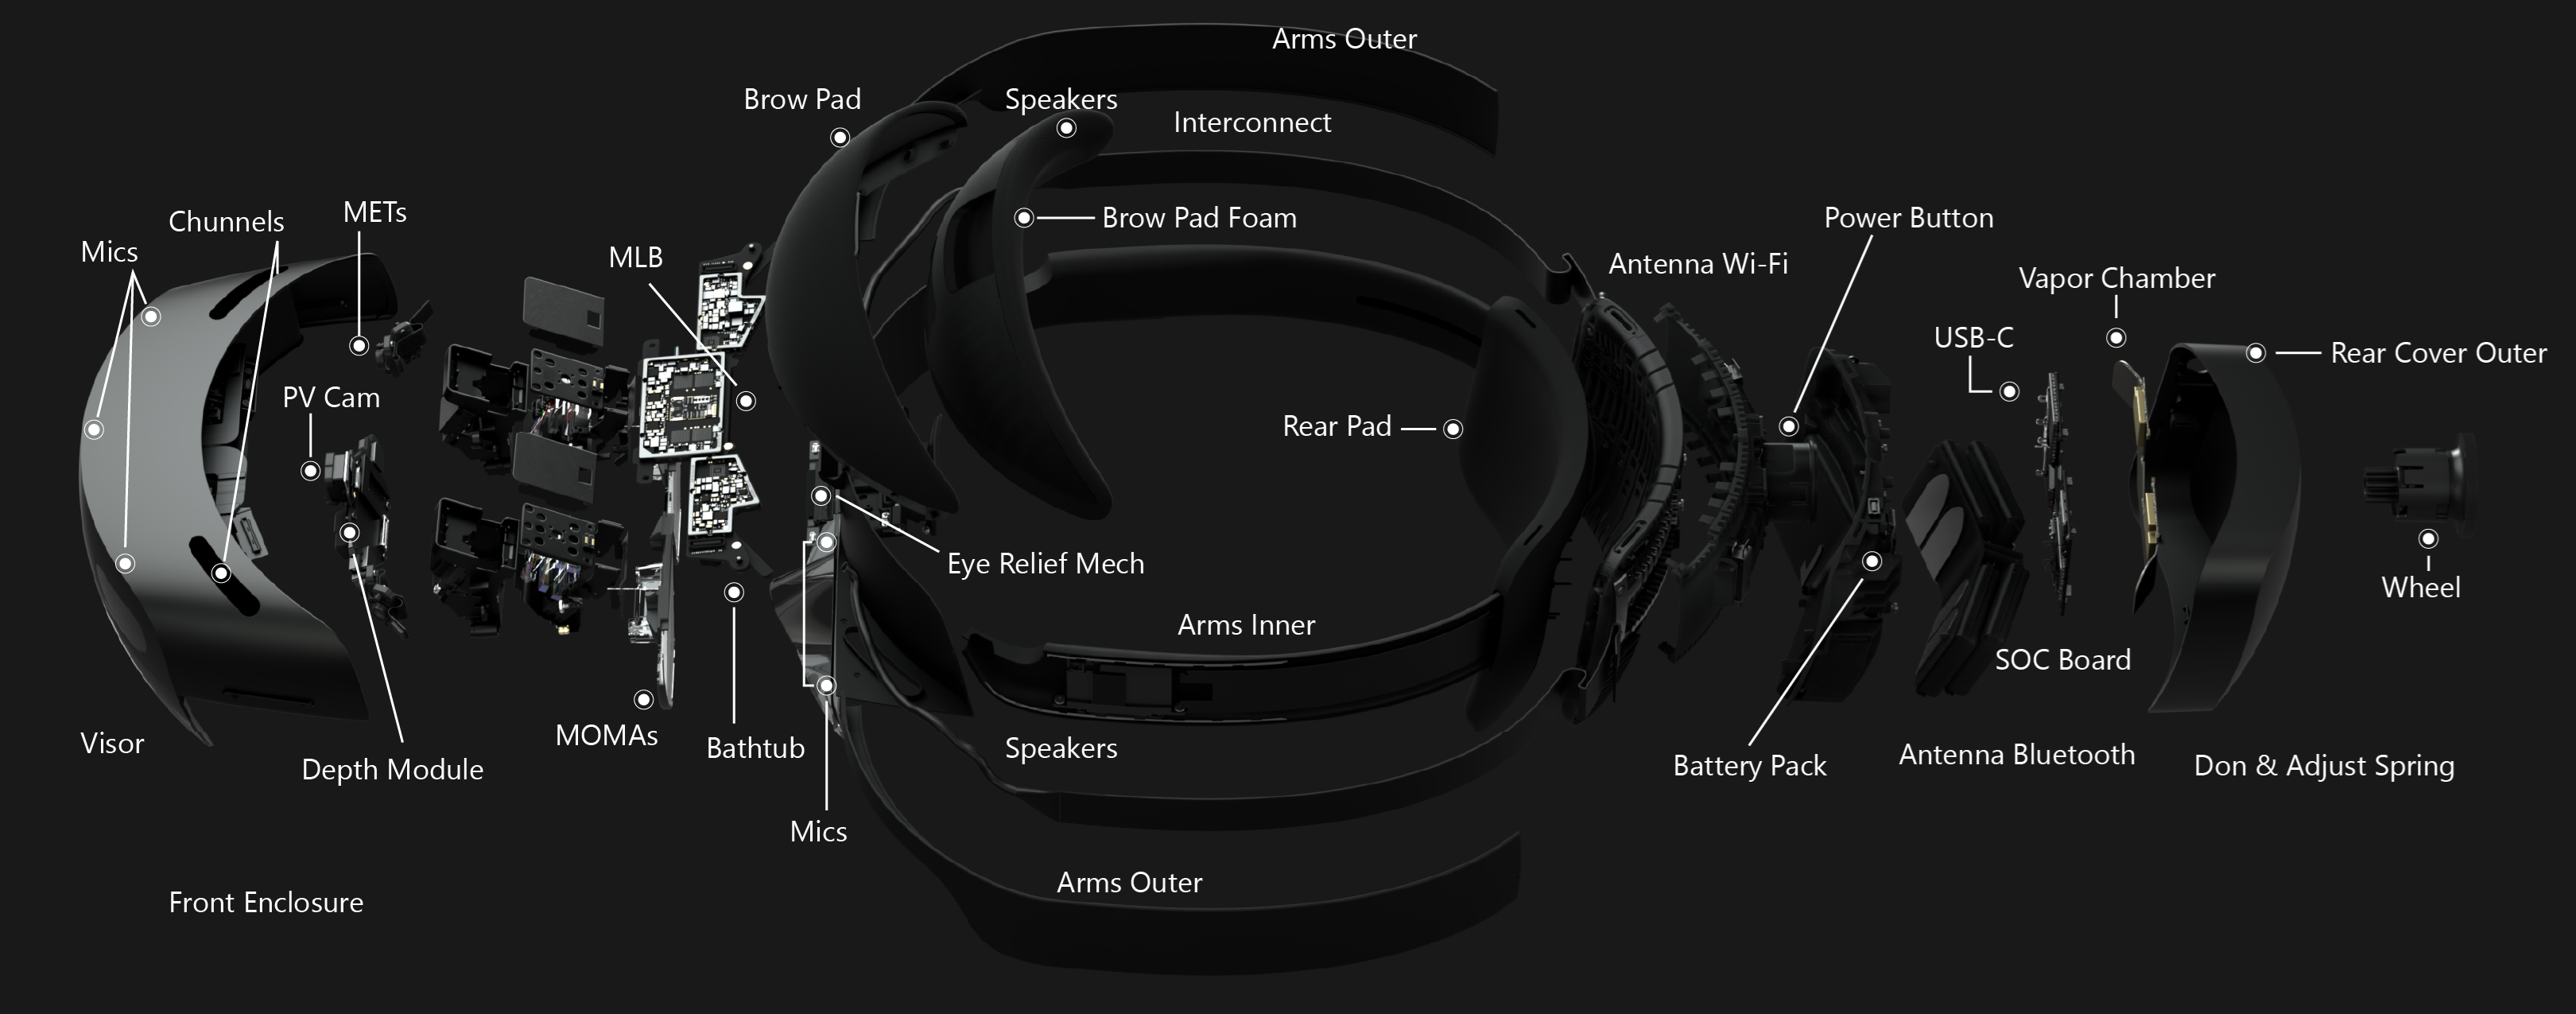
\includegraphics[width=\textwidth]{obrazky-figures/ar/hololensDescription.png}
	\caption{Rozebrané brýle Hololens 2 s popisky jednotlivých částí. Převzato z \cite{hololens2ms}.}
	\label{pic:hololens2}
\end{figure}


\subsubsection{Modalita/vstup od uživatele}
S rozhraním v brýlích se dá interagovat několika způsoby. Autor je seřadil podle obvyklé frekvence užití v aplikacích.
\begin{enumerate}
    \item Gesta a pohyb rukou - Jedná se o hlavní cestu pro interakci s prostředím. Brýle dokáží rozpoznat přesný pohyb rukou včetně pohybu prstů. Díky tomu lze provádět různá gesta v prostoru a tím interagovat s okolím. Ovládání je velmi intuitivní, protože můžete na jednotlivé objekty "fyzicky sahat". Pokud má aplikace engine na fyziku, můžete z objekty i házet či jinak užívat fyzické vlastnosti objektů. Ukázka funkcionality je na obrázku \ref{pic:hololens2Demo}.
   \item Pohyb v prostoru a pohyb hlavy - Rozhraní lze naprogramovat, aby interakce s prostředím probíhala díky pohybu uživatele v prostoru. Lze tedy implementovat, aby jednotlivé objekty reagovaly například po pohledu na objekt. 
    \item Hlasové ovládání - Díky integrovaným mikrofonům a jednotce pro rozpoznávání řeči lze brýle ovládat hlasovými příkazy. Syntezátor hlasu naopak může k uživateli promlouvat díky integrovaným reproduktorům v zadní části brýlí.
    \item Pohyb očí - Díky snímání pohybu očí může například rozhraní reagovat při pohledu na určitý objekt. Při testování autor shledal, že je pohyb očí zaznamenán poměrně přesně. Pro jemnou interakci však nestačí.
 
    \item Externí zařízení - I když brýle lze užívat pouze za pomocí výše zmíněného, uživatel má možnost si pomocí Bluetooth a Wi-Fi připojit vlastní periferie, jako je klávesnice, myš nebo třeba gamepad. 
\end{enumerate}
\begin{figure}[ht] 
	\centering
	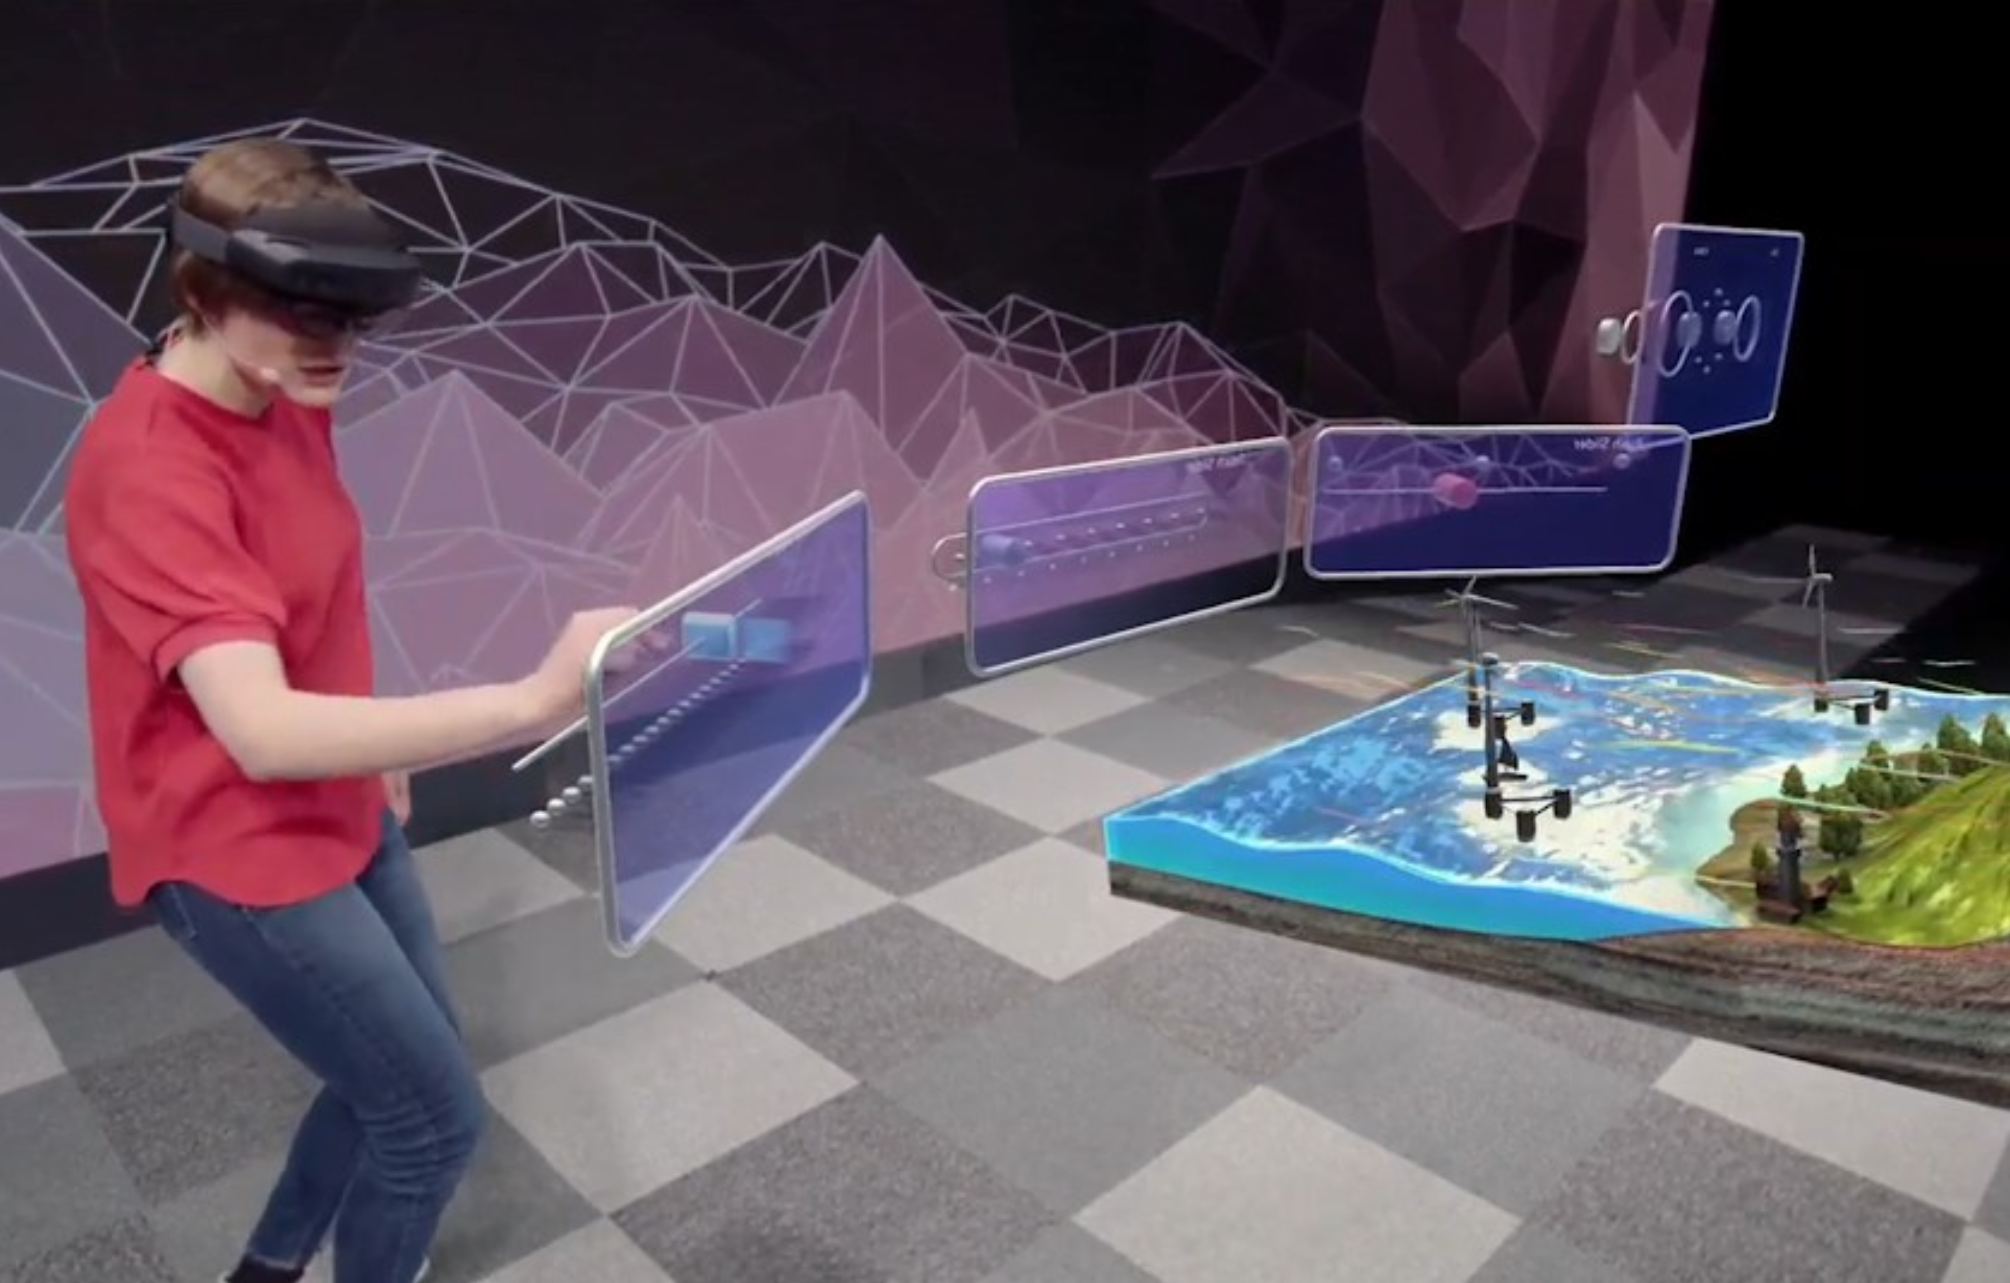
\includegraphics[width=0.95\textwidth]{obrazky-figures/ar/hololensDemo.png}
	\caption{Ukázka ovládání scény za pomocí gest. Převzato z video dema \cite{hololens2videoDemo}}
	\label{pic:hololens2Demo}
\end{figure}

\subsubsection{Souhrn technických limitací brýlí}
I když jsou brýle napěchované moderními technologiemi a autorovy přijdou jako "malý technický zázrak", mají své limitace. Proto je zde uveden souhrn limitací, které autor bral v potaz při tvorbě práce. 
\begin{itemize}
    \item Malé zorné pole - I když byl rozsah zorného pole vylepšen, je pořád velmi malý - 52°.  Zdroj \cite{HumanEye} uvádí, že je člověk schopen vnímat až 190° v horizontálním rozsahu a 100° vertikálním rozsahu. Z toho plyne že je nutné rozhraní nutné smrštit co ke středu pomyslné zorné linie. Užít vizualizace v periferní vidění je tedy proto nemyslitelné. Vizualizace omezení je na obrázku \ref{pic:hololens2Fov}.
    \item Nepřítomnost GPS modulu - Brýle nemají žádnou jednotku pro lokalizaci uživatele. Při spuštění brýlí je uživatel umístěn na nulové souřadnice. Z toho vyplývá, že brýle využívají vlastní souřadnicový systém. Vizualizace pro zobrazení drona se s tímto faktorem musí vyrovnat.
    \item ARM architektura - Protože brýle běží na architektuře ARM je nutné užít implementační platformu UWP (Univerzal Windows Platform). Proto je nutné používat při vývoji pouze knihovny podporující tuto platformu. Integrace ostaních knihoven není možná.
    \item Mapování prostoru - Brýle neobsahují žádnou databázi o podobě okolí. Okolí si brýle modelují za pomocí kamer a to pouze ve velmi blízkém okolí (cca rádius 10m od uživatele). Toto okolí nemusí být vytvořeno dokonale a tudíš se na něj nelze spolehnout. Pro využití v kontextu vizualizace drona je velmi limitující.
    \item Konektivita - brýle mají integrovaný Wi-Fi a Bluetooth modul. Pouze za pomocí těchto technologií lze brýle připojit k dalším zařízením. Použití Bluetooth komunikace by v práci vedla na velkou implementační náročnost, které neodpovídá povaha projektu, proto bude komunikace přes Wi-Fi modul preferována. Wi-Fi na více podporuje lepší přenosové rychlosti a lepší variabilitu. 
    
    Wi-Fi modul nelze užít jako přístupový bod (zkratka AP), což brýle odsuzuje k závislosti na externím Wi-Fi AP. Při vývoji proto bude nutné počítat s přítomností tohoto hotspotu. 
\end{itemize}
\begin{figure}[ht] 
	\centering
	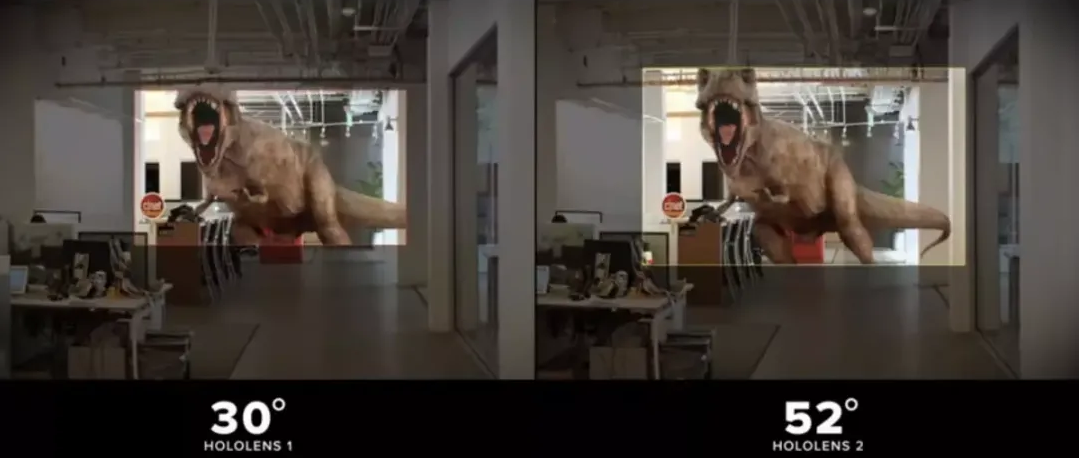
\includegraphics[width=0.85\textwidth]{obrazky-figures/ar/Hololens-2-fov.png}
	\caption{Ukázka limitace zorného pole. Převzato z \cite{hololens1/2difrences}}
	\label{pic:hololens2Fov}
\end{figure}

\chapter{Drony a jejich použití }
Drony, formálně pojmenované UAV (unmanned aerial vehicle), jsou obecně letadla bez pilota, posádky či pasažérů na palubě letounu. Tento letoun je pak řízen dálkově či může být řízen plně autonomně palubním počítačem \cite{UAVMeaning}. 

Koncept dronů sahá až do 19 století, kde bylo poprvé  zaznamenáno jejich nasazení. Jednalo se o horkovzdušné balóny vybavené výbušninami, které byly shazovány za pomocí časové zápalky (viz. obrázek \ref{pic:balon}). Roku 1839 Rakousko použilo tuto zbraň při útoku na Benátky. Velký průlom v této oblasti byl zaznamenán v první světové válce, kdy vznikl "Hewitt-Sperryův automatický letoun", jeden z prvních radiem ovládaných letounů (viz. obrázek \ref{pic:autoPlane}). Další velký pokrok přišel v druhé světové válce, kdy drony začaly ukazovat svůj velký potenciál jak na bojišti, tak v tréningových oblastech pro výcvik.

Přestože bylo za války vyrobeno nepřeberné množství těchto dronů, lidé byly kvůli jejich špatné spolehlivosti velmi skeptičtí, což vedlo ke zpomaleni vývinu a tak další pokrok přicházel až v době války ve Vietnamu a během studené války. \cite{DroneHistory,DroneHistory2WWX,DroneKatogorySouhrn,DroneHistory3} 

Tato historie se spíše stahovala k vývoji bezpilotním letounům (to jsou motorové letadla těžší než vzduch, používající ke svému pohybu aerodynamických sil, s pevnými nosnými plochami). Drony pro civilní použití, jak je známe dnes jsou však spíše multi-rotorové stroje. První pokus o vytvoření takovéhoto stroje se připisuje designérovy Louis Breguetovy, jenž navrhl první takovýto stroj (viz. obrázek \ref{pic:quadrocopter}). Po sestavení stroje bylo poznamenáno, že stroj několikrát letěl \cite{Quadcopter}. Rozšířené užití designu multi-rotorové stroje  na poli civilním trhu s drony je dle zdroje \cite{DroneHistory3} zaznamenáno v prvním desetiletí 21. století. Od těchto dob se technologie dronů neustále vyvíjí a to především  v oblasti pohodlnosti použití, spolehlivosti a levnější výroby.


\begin{figure}[ht]
    \centering
    \begin{subfigure}[t]{0.27\linewidth}
        \centering
        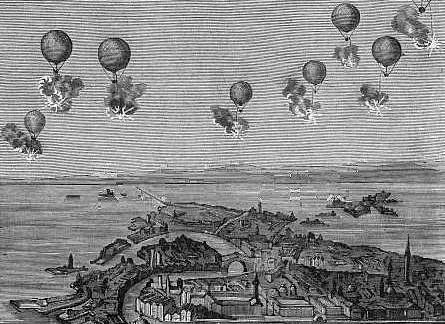
\includegraphics[width=\linewidth]{obrazky-figures/drony/history-of-drones-balloons.jpg}
        \caption{Ilustrace nejstarších dronů. Převzato z \cite{DroneHistory}.}
        \label{pic:balon}
    \end{subfigure}
    \hfill
    \begin{subfigure}[t]{0.26\linewidth}
        \centering
        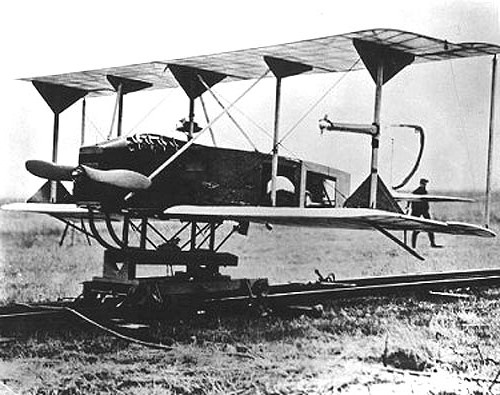
\includegraphics[width=\linewidth]{obrazky-figures/drony/hewitt-sperry_automatic_airplane_1918.jpg}
        \caption{Hewitt-Sperryův automatický letoun. Převzato z \cite{DroneHistory2WWX}.}
        \label{pic:autoPlane}
    \end{subfigure}
        \hfill
    \begin{subfigure}[t]{0.43\linewidth}
        \centering
        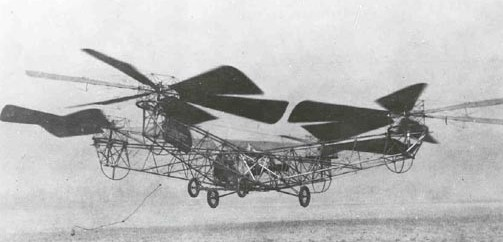
\includegraphics[width=\linewidth]{obrazky-figures/drony/Bothezat_Quadrotor.jpg}
        \caption{Quadrokoptéra de Bothezat helicopter. Převzato z \cite{Quadcopter}.}
        \label{pic:quadrocopter}
    \end{subfigure}
    \caption{Průlomové historické stroje v oblasti technologie dronů.}
    \label{pic:historymisc}
\end{figure}


\section{Moderní civilní drony} \label{sec:modCivDrony}
Jak již bylo řečeno, na civilním trhu dronů nejčastěji nalezneme multirotorové stroje, nejčastěji 4 rotorové kvadrokoptéry. Vyrábějí se i více rotorové varianty drony, které mohou díky přidaným rotorům poskytnout větší zvedací výkon a redundanci pro případ selhání jednoho či více pohonných systémů \cite{Multirotor}. 

Multirotorový design je v oblasti dronů oblíbený, protože umožňuje kolmý start a vznášení se namístě. Zároveň nevyžaduje složité mechanizmy, jako je cyklika a kompenzační rotory jako je tomu u klasických vrtulníků. Každá pohonná jednotka dronu je identická a ovládání dronu je uskutečněno díky regulaci výkonu jednotlivých rotorů. I když jsou pohonné jednotky identické, pro vyrušení nežádoucích rotačních momentů je potřeba zajistit, aby sousední rotory měli vrtule s obráceným stoupáním a otáčeli se opačně (proto málo kdy naleznem drony s lichým počtem rotorů)\cite{Quadcopter}. Obrázek drona užitého při vývoji viz. \ref{pic:mavicMini}.

Jelikož je potřeba rychle regulovat výkony motorů pro korektní řízení dronu, je ideálním kandidátem pro pohon elektrický proud. Jeho dodávku obvykle zajišťuje akumulátor Li-Po nebo Li-Ion. Tyto akumulátory by měli být ohodnoceny vysokou hodnotou C (tato hodnota značí jaké množství energie je schopna bezpečně dodat) \cite{bateriesDron}.

Udržení drona stabilně ve vzduchu je složitý úkol, proto dron disponuje sadou senzorů, mezi nejnutnější patří gyroskop a akcelerometry (celý systém se nazývá IMU) s jejichž pomocí je možné dron stabilizovat. Pro přesné držení polohy dron na více potřebuje přijímač GPS, elektronický kompas a výškoměr. Výškoměr je obvykle u dronů optický, kvůli nízkým pořizovacím nákladům. U dražších dronů můžeme nalézt i barometr. Optické čidlo může být také využito pro korekci polohy drona, jako je tomu u dronu DJI. Optická čidla se navíc nově používají pro detekci překážek. Kvůli těmto optickým senzorům se nedoporučuje létat s dronem za snížených viditelnostních podmínek. Pro správnou funkci potřebují čidla před letem zkalibrovat, často tak budete muset provádět kalibraci kompasu a jednotky IMU. Výstupy těchto senzorů spolu se vstupy od uživatele z vysílačky jsou následně zpracovány letovým počítačem a výstupem jsou úrovně výkonu pro jednotlivé regulátory motorů \cite{droneSenzors}.

Moderní drony z pravidla obsahují kameru pro nahrávání a přenos obrazu směrem k pilotovy. Tato kamera může být fixně umístěná - tuto variantu nalezneme například u FPV dronů. Druhou častější variantou je upevnění kamery do gimbal stativu, který stabilizuje kameru, aby výsledný obraz byl plynulý a vyhlazený. Často je tento mechanizmus obohacen o optickou stabilizaci, pro ještě lepší požitek z videa. Tato jednotka se u menších dronů nachází ve předu dronu. U filmařských dronů se tato jednotka nachází na spodku dronu přesně ve středu drona a to z důvodu váhy kamery, která by drona mohla destabilizovat. Tento design obvykle doprovází zvedací podvozek, aby nezavázel ve scéně kamery.


\begin{figure}[h]
  \begin{minipage}{0.5\textwidth}
    \centering
    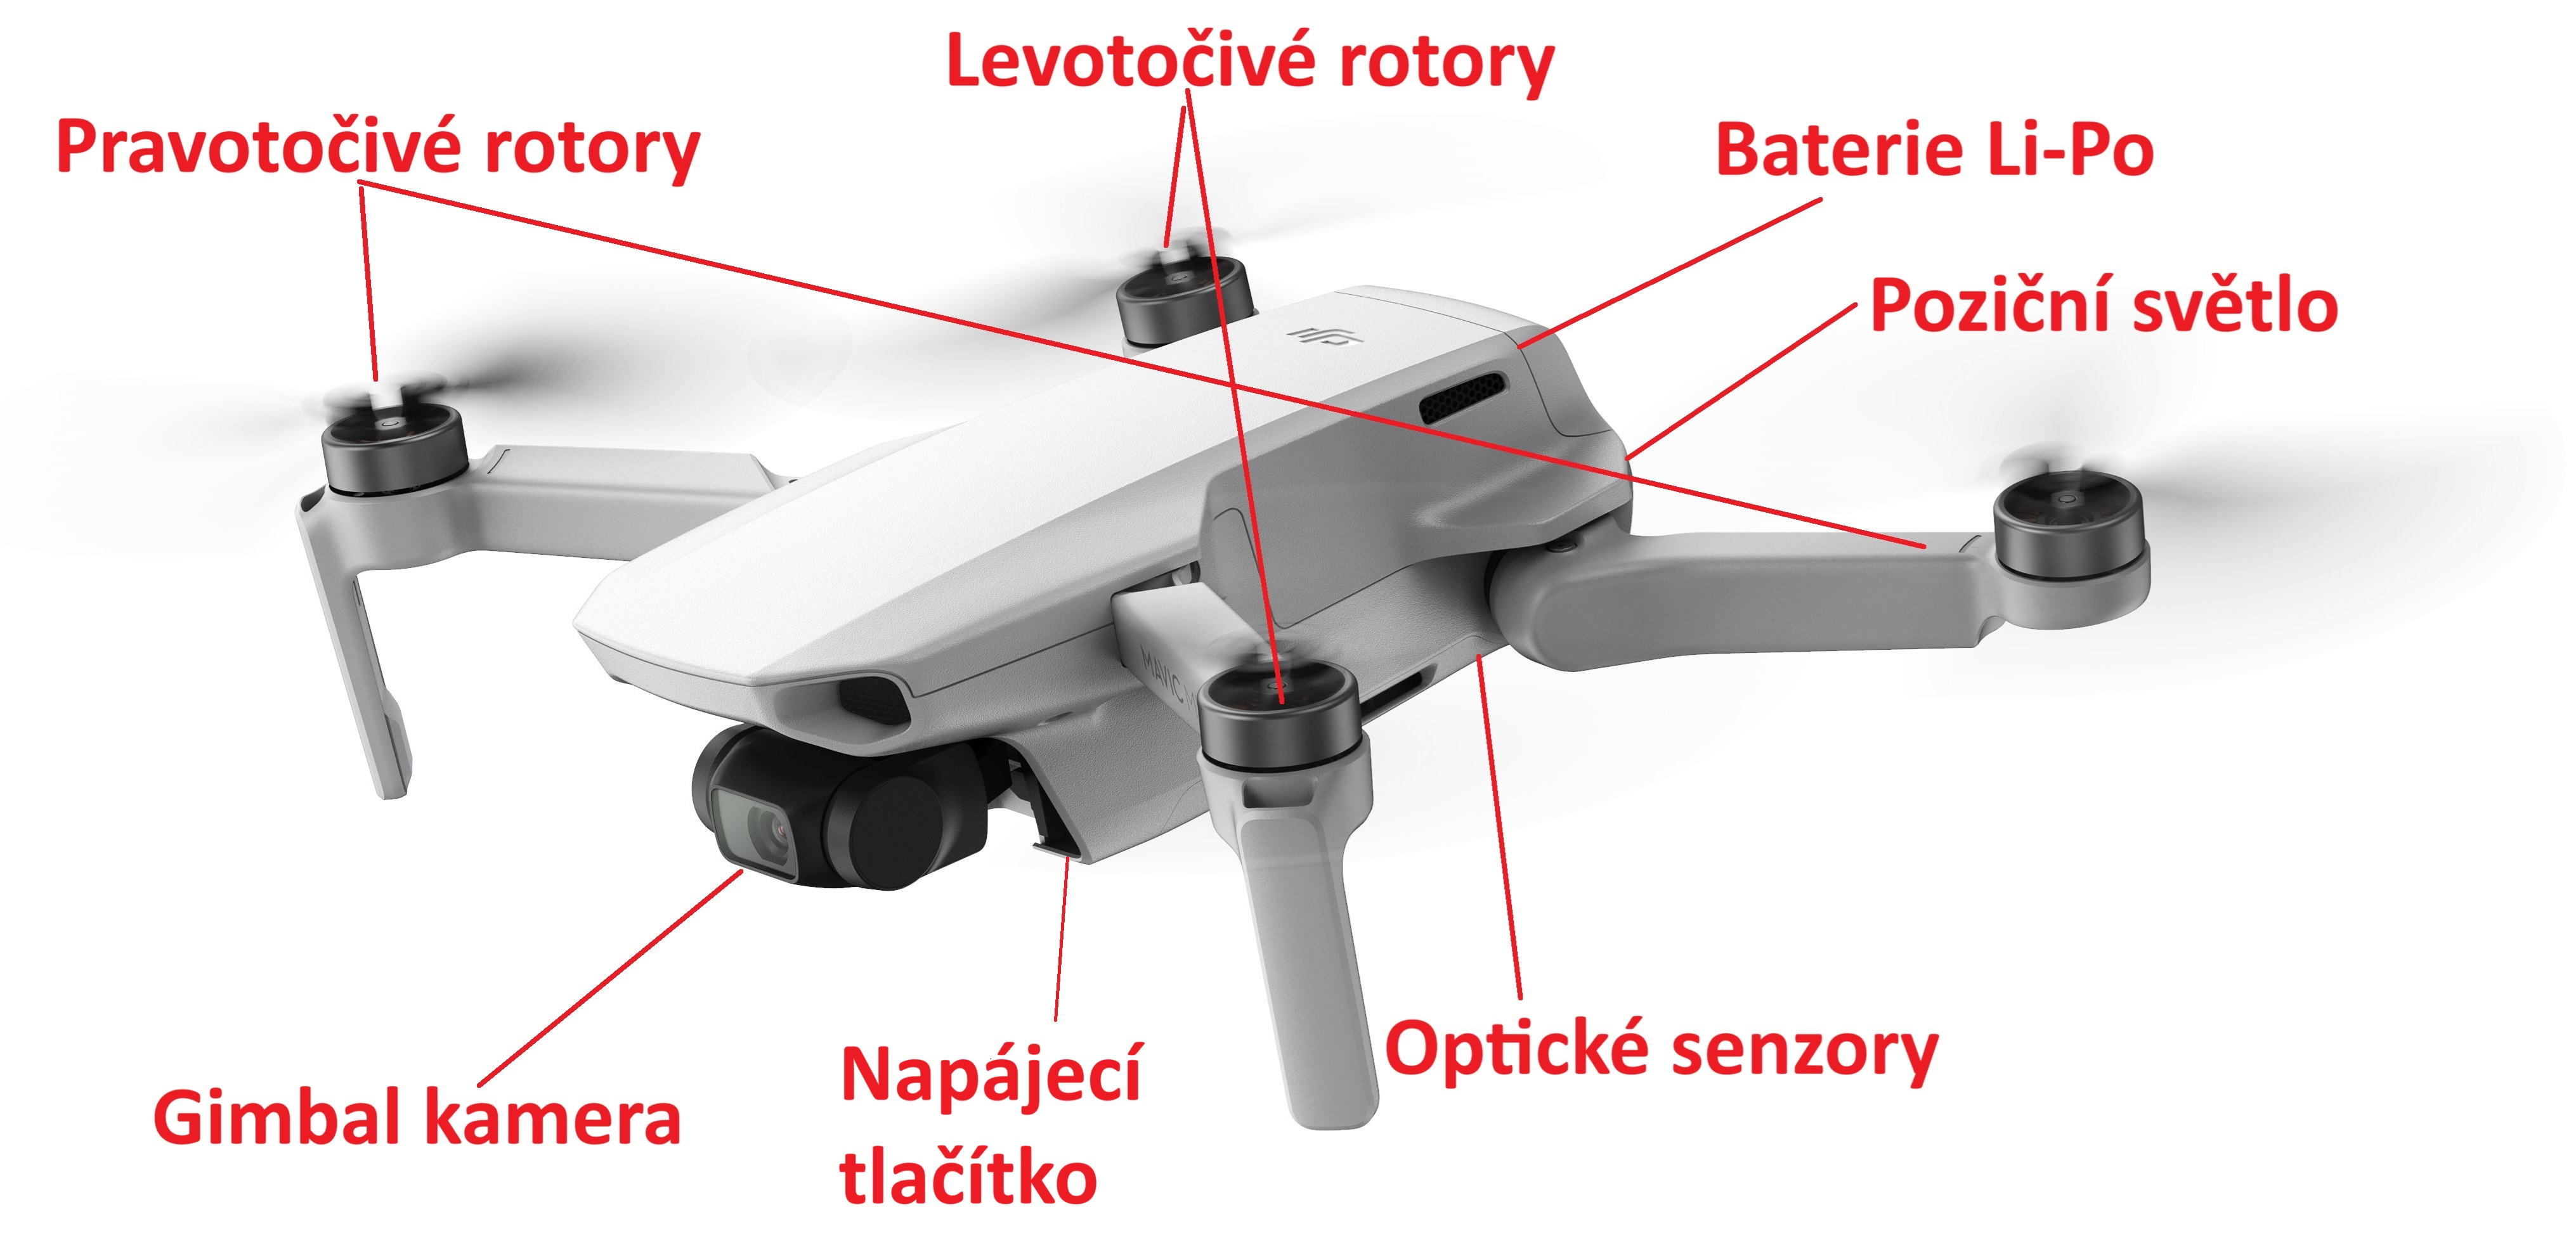
\includegraphics[width=\textwidth]{obrazky-figures/drony/djiMavicMiniPopis.jpg}
    \caption{Ukázka dronu Mavic Mini 2 \\využitého pro vývoj. Převzato z \cite{mavici2pic}.}
    \label{pic:mavicMini}
  \end{minipage}
  \begin{minipage}{0.45\textwidth}
    \centering
    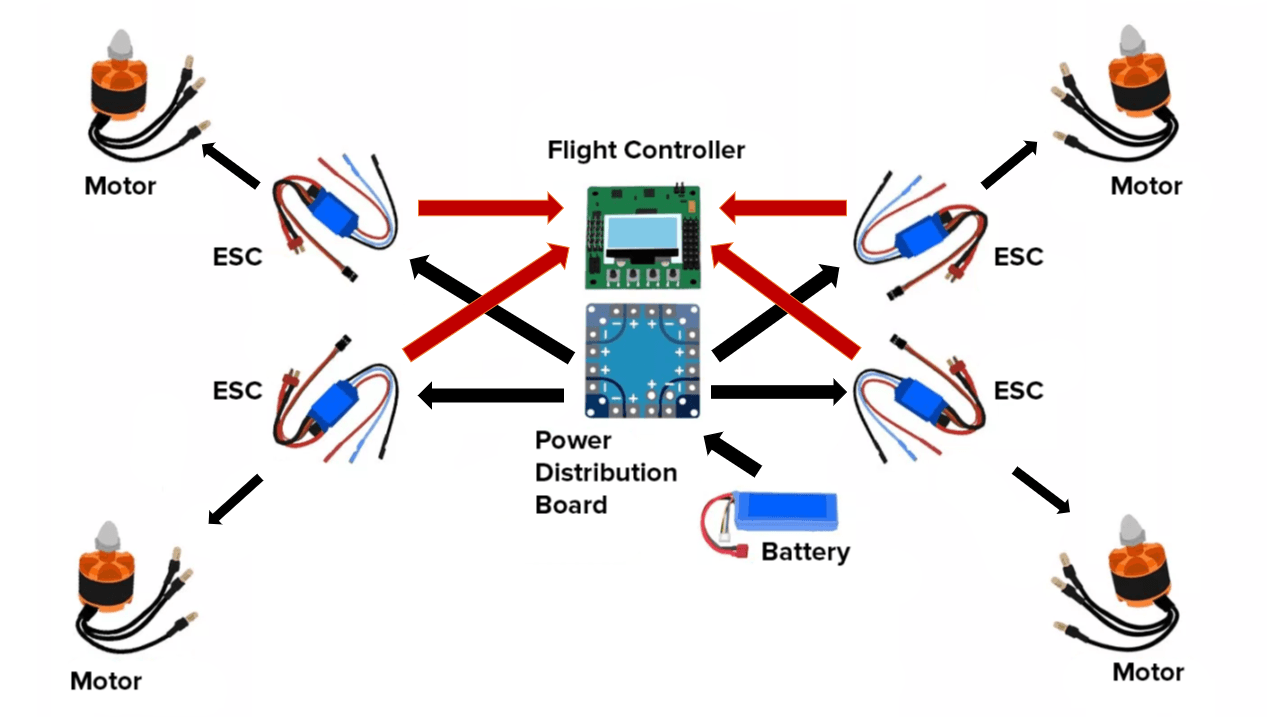
\includegraphics[width=\textwidth]{obrazky-figures/drony/DroneIntenals.png}
    \caption{Schéma zapojení součástek dronu. Převzato z \cite{droneIntrnals}.}
    \label{fig:dronSchema}
  \end{minipage}
\end{figure}

\section{Prostředky pro ovládání dronů} \label{sec:ovladace}
\subsubsection{Pákový ovladač}
V dnešní době se většina civilních dronů ovládá za pomocí 2 pákových joysticků neboli 4 os. Každá osa má přiřazený směr pohybu drona dle zvoleného ovládacího módu (obvykle můžete módy přepínat v ovladači). Standardně se používají módy 4 (viz. obrázek \ref{pic:pakaMody}). Mód zde popsaný bude mód 2, protože se v kontextu dronů používá nejvíce. V tomto módu má levý joystick funkci zvyšování a snižování výšky ve vertikální ose. V horizontální ose se ovládá rotace dronu doleva/doprava. Pravým joystickem se ovládá pohyb v před/vzat na vertikální ose, pohyb doprava/doleva se ovládá na horizontální ose. Při pohybu joysticků do krajních poloh směrem k sobě dron odstartuje (pouze u dronů DJI).

Ovládání dronu je díky stabilizačním asistentům drona jednoduché, pokud budou joysticky ve středové poloze, dron zastaví a bude se vznášet na místě. Rychlost reakce drona na změny polohy pák se liší dle zvoleného módu letu. V mód Position dron jemně mění svou pozici, v módu Sport reaguje rázněji a létá vyššími rychlostmi. V posledním módu Cinematic dron létá velmi plynule.

Ovladač často obklopují pomocné ovládací prvky, na ovladači drona použitého k vývoji je na vrchní straně ovladače přítomna sada dvou tlačítek. Jedno slouží pro návrat do oblasti vzletu, druhé slouží k zapnutí vysílače. Na zadní straně je přítomno tlačítko pro pořízení fotky a videa. Je zde také roller ovládající pohyb gimbalu ve vertikální ose. Hight-end ovladače obsahují i integrovaný displej pro zobrazení videa z drona. Levnější tuto možnost poskytují přes připojený mobilní telefon. Příklad ovladače je na obrázku \ref{pic:paka}.
\begin{figure}[h]
  \begin{minipage}{0.55\textwidth}
    \centering
    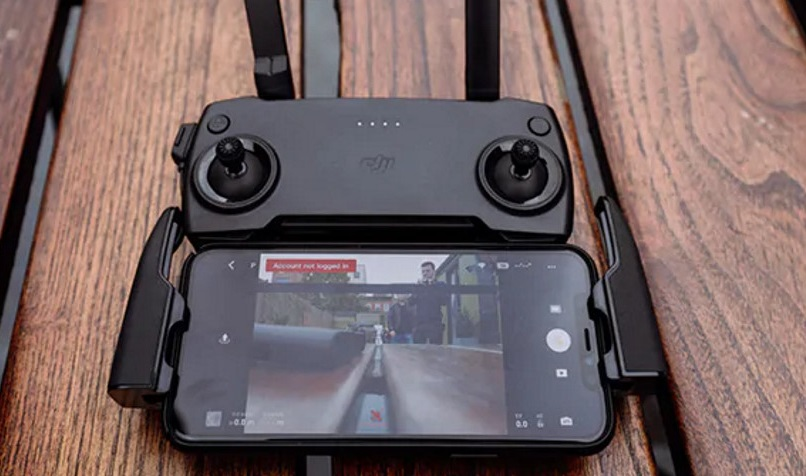
\includegraphics[width=\textwidth]{obrazky-figures/drony/controler.jpg}
    \caption{Ovladač Mavicu Mini 2.\\ Převzato z \cite{pakaOvladac}.} % popsat obrázek
    \label{pic:paka}
  \end{minipage}
  \hfill
  \begin{minipage}{0.4\textwidth}
    \centering
    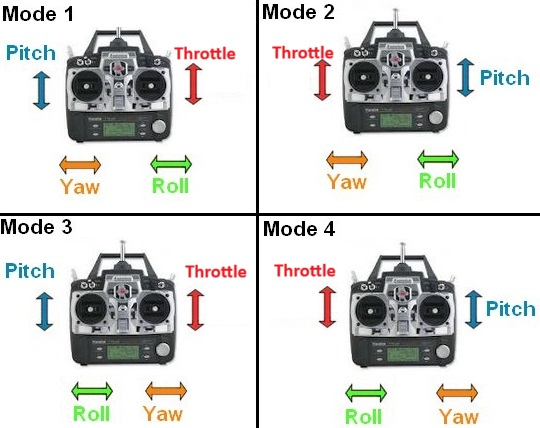
\includegraphics[width=\textwidth]{obrazky-figures/drony/transmiterMods.jpg}
    \caption{Módy pákového ovladače. Převzato z \cite{pakaMody}.} % to do zvětšit obrázek
    \label{pic:pakaMody}
  \end{minipage}
\end{figure}

\begin{figure}[h]
  \begin{minipage}{0.6\textwidth}
  \subsubsection{DJI Motion 2 }
    Jedná se o nový ovladač, který v kombinaci s brýlemi je určen pro řízení FPV dronů. Je specifický tím, že se dá ovládat pouze jednou rukou. Směr kupředu ovládáte spouští ovladače. Stoupání a zatáčení se ovládá náklonem ovladače. Dodatečné pohyby lze provést mini joystickem. Tento ovladač je zmíněn díky možnosti ovládání pouze jednou rukou, což by usnadnilo manipulaci s objekty v prostředí AR. 
  \end{minipage}%
  \hfill
  \begin{minipage}{0.38\textwidth}
    \centering
    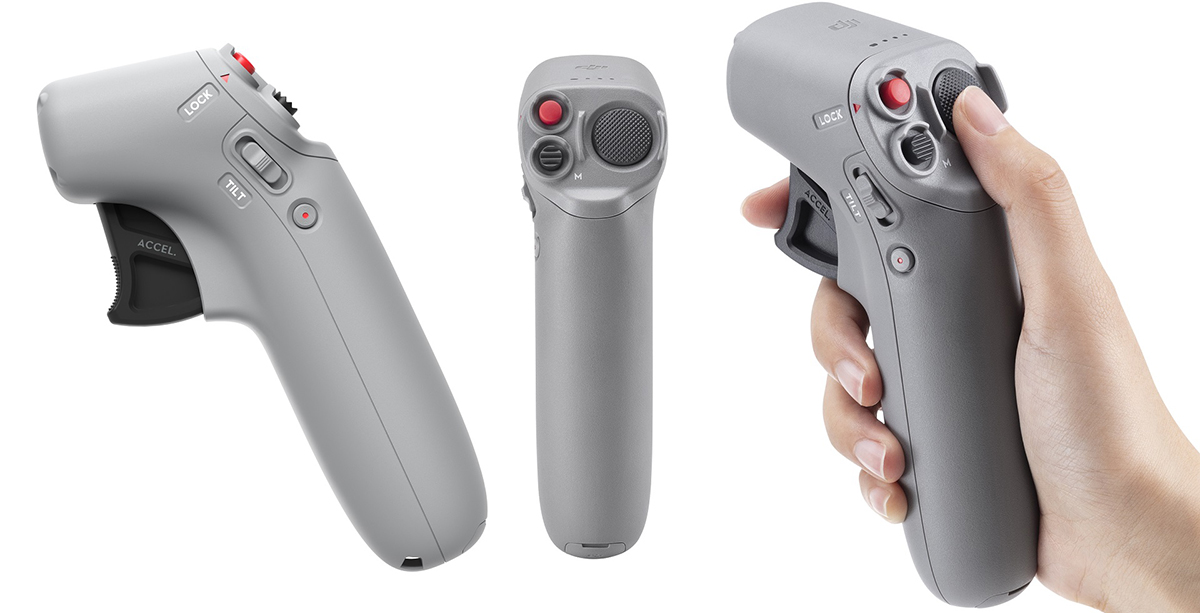
\includegraphics[width=\textwidth]{obrazky-figures/drony/djiMotion.png}
    \captionsetup{type=figure} % Set up for figure caption outside of float
    \caption{Ovladač DJI Motion~2. Převzato z \cite{djiMotionPic}.}
    \label{fig:DjiMotion}
  \end{minipage}
\end{figure}
\newpage
\section{Legislativa a pravidla pro civilní létání z drony}
V průběhu posledních let, zvláště od období masivního rozšíření dronů mezi širokou veřejnost došlo k značným úpravám v legislativě pro provoz dronů. Tyto nová nařízení měli zajistit bezpečnější provoz dronů ve veřejném vzdušném provozu a zajistit respektování občanského soužití. Tyto pravidla se musí při létání striktně dodržovat, aby se předešlo zbytečným nehodám a incidentům. Proto autor uznal za vhodné tyto pravidla nastudovat a rozebrat nejzásadnější body. Tento rozbor bude dále využit při návrhu aplikace.

Rozbor je aktuální k začátku roku 2024.

\subsection{Kategorie dronů}
Provozování drona se dle účelu použití dělí na 3 hlavní kategorie: Open, Specific a Certified. Tyto kategorie se liší hlavně rizikem použití. Nejvíce pozornosti bude věnováno kategorii Open, protože je nejvíce relativní k povaze práce.

\subsubsection{Specific}
Tato kategorie zahrnuje operace dronů se středním rizikem. Patří sem operace, které vyžadují prolomení limitací kategorie Open. Příkladem může být let bez přímé viditelnosti na drona, let 120m nad zemí, odhození materiálu, překročení maximální letové hmotnosti 25 kg nebo lety s těžkými drony nad zástavbami\cite{EASA:SpecificCategory}. 
    
Pro tuto kategorii byly vytvořeny dva standardní scénáře užití, které nepotřebují autorizaci od AESA. Jedná se o scénář letu typu VLOS (létání při přímé viditelnosti na drona) a BVLOS (létání bez přímé viditelnosti na drona). Pokud aktivita nespadá do těchto scénářů je potřeba povolení od EASA \cite{DroneKatogorySouhrn,EASA:SpecificCategory}.  
    

\subsubsection{Certified} 
Kategorie zahrnuje vysoce rizikové použiti dronů. Do kategorie například patří provoz bezpilotních nákladních letadel, doručovací drony nebo vzdušné taxi. Jak název napovídá, všechny tyto aktivity musí být certifikovány od EASA\cite{EASA:CertifiedCategory}.

\subsubsection{Open} 
Tato sekce vzešla ze zdrojů \cite{EASA:openSouhrn2024,AlzaDronyKategorie,DroneKatogorySouhrn}. Kategorie Open je dostupná pro širokou veřejnost, určena je pro operace s nízkým rizikem. Na provoz drona v této kategorii nepotřebujete povolení od organizace AESA. Kategorie Open se dále dělí na podkategorie A1, A2 a A3. Pro pilotáž dronů v kategorii A1/A3 se musíte registrovat na webu ÚCL (úřad civilního letectví) a absolvovat online školení. Pro kategorii A2 na více musíte mít certifikaci. V kategorii A2/A3 musíte mít sjednané povinné ručení dle podmínek kategorie.


Od roku 2024 každý nově prodaný dron musí být klasifikován do tříd C0-C4. Třídy lze přímo namapovat na podkategorie Open, ale je možné létat s dronem nízké kategorie podle pravidel vyšší kategorie (A3). Drony neoštítkované kategorií C, které byly prodány před rokem 2024 lze zařadit do třídy A1 pokud jejich letová hmotnost nepřesáhla 250g, jinak jsou zařazeny do kategorie A3.

Kategorizace slouží k minimalizování rizika střetu s osobami. Nad lidmi a v zástavbě můžete bez licence létat pouze s nejlehčími drony, s licencí můžete létat i s mírně těžšími drony. Provoz velmi těžkých dronů (>4 Kg) je možný pouze daleko od lidí a zástavby. 

\paragraph{Jednotlivé podkategorie Open:}
\begin{itemize}
    \item A1 - s dronem se smí létat nad lidmi, ale nesmíte létat nad skupinami lidí. Do této kategorie spadají třídy C0 a C1. Pro pilotáž dronů v této kategorii se budete muset zaregistrovat na webu ÚCL a složit online test. Vyjmou jsou dětské hračky nevybavené kamerou. Tyto drony můžete provozovat také v kategorii A3.

    \item A2 - s těmito drony nesmíte letět blízko lidí. Do této kategorie spadá třída dronů C2. Na tuto kategorii musíte absolvovat školení spolu s certifikačním procesem pro získání licence A2. Tato skupina je určená pro létání v zástavbě s těžšími drony.
    \item A3 - do této kategorie automaticky patří všechny drony třídy C3 a výše (hmotnost do 25 kg), dále pak drony soukromě postavené a drony neoštítkované prodané před rokem 2024 s letovou hmotností nad 250g. S těmito drony musíte létat daleko od lidí a zástavby.
\end{itemize}

\paragraph{Jednotlivé třídy dronů:}
\begin{itemize}
    \item C0 - Nejmenší drony (hmotnost do 250g) s maximální rychlostí do 68 km/h a napájením do 24V. Příkladem může být dron Mavic Mini 2 který byl použit pro vývoj. 
    \item C1 - Drony vážící do 900g s maximální rychlostí do 68 km/h, napájením do 24V. Obsahují více bezpečnostních prvků než kategorie C0 a hluk je limitován 85 dB.
    \item C2 - Drony vážící do 4 Kg, stejné povinné bezpečnostní prvky jako u C2, na více musí ale obsahovat Low Speed mode (3m/s), aby se mohl pohybovat v blízkostí lidí. Hlučnost je omezena do 97 dB a pohon je limitován 48 V.
    \item C3 - Drony do 25 Kg a musejí se vejít do rozměru 3m. Pohon do 48 V.
    \item C4 - Je určena pro modely letadel, stahuje se na ní pouze váhové omezení (<25Kg) a je zde zakázán autonomní režim. 
    \item C5/C6 - Podobné C3 s přidanými bezpečnostními prvky.
\end{itemize}


\begin{figure}[ht]
	\centering
	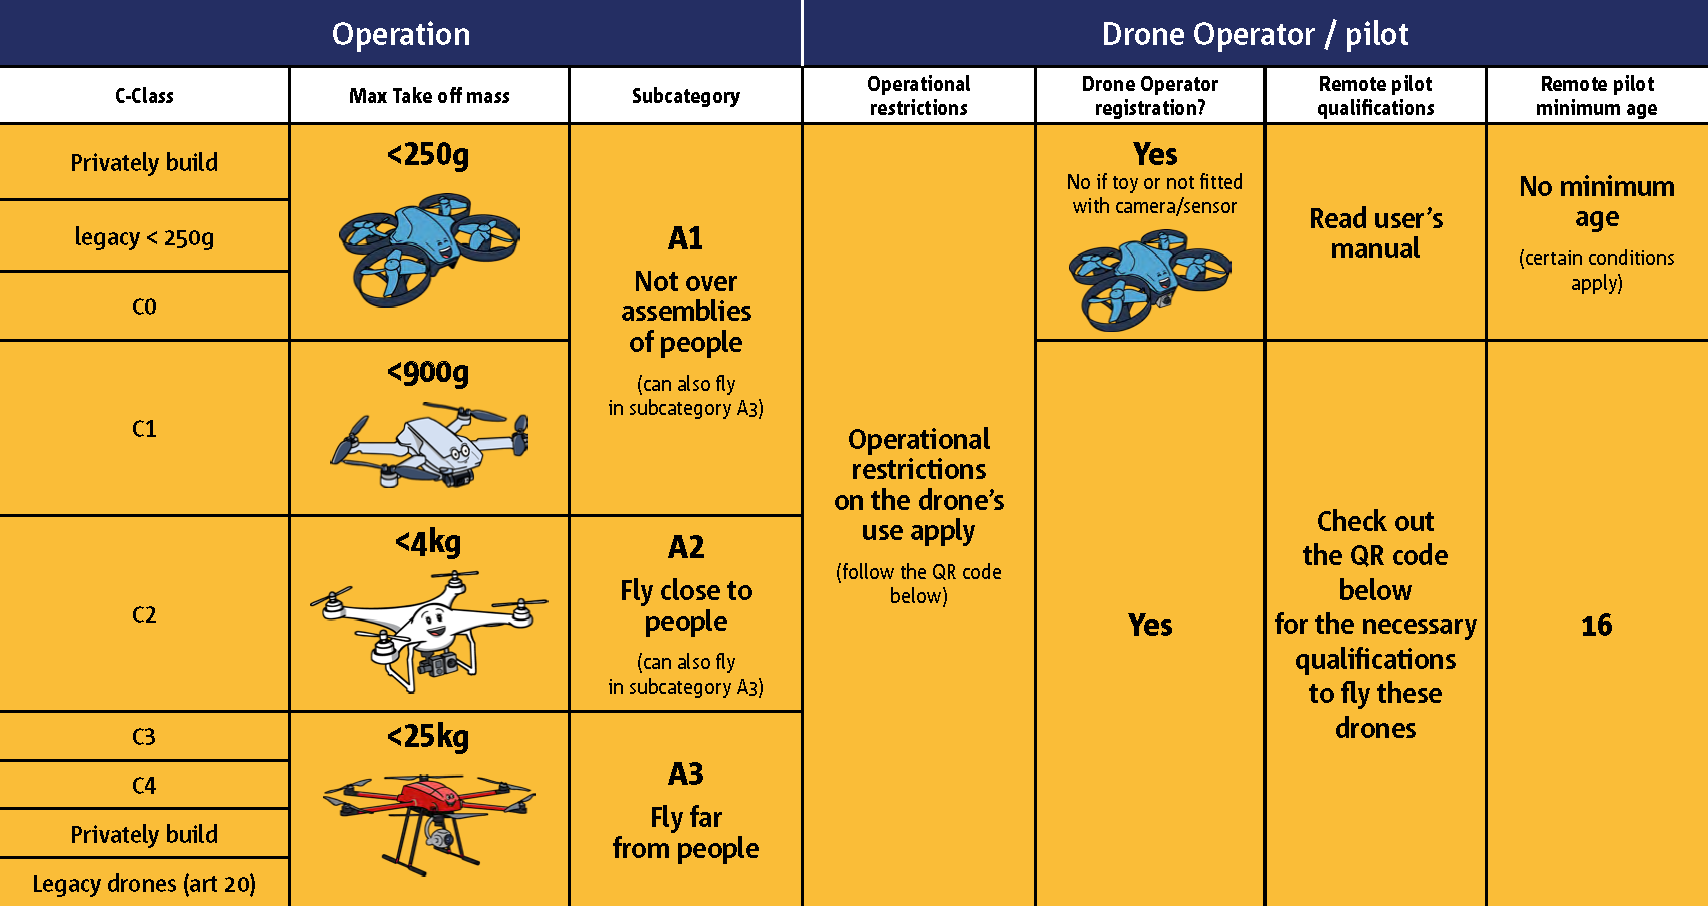
\includegraphics[width=0.81\textwidth]{obrazky-figures/drony/droneCatTable.png}
	\caption{Přehledová tabulka kategorií dronů a podkategorií Open.  Zdroj \cite{EASA:openSouhrn2024}.}
	\label{covpitDrLiner}
\end{figure}


\paragraph{Předstartovní procedura typického dronu}
Vývoj v oblasti dronů značně zjednodušil užívání dronů a proto pro mnohé uživatele navodil falešný pocit robustnosti dronů. Drony jsou i přes veškerá zjednodušení pořád velmi sofistikovaná a křehká zařízení, které je potřeba provozovat s respektem. Proto autor sepsal několikabodový checklist, který by zodpovědný operátor drona měl dodržovat.  Procedura je psaná pro dron DJI Mavic Mini 2, ale není problém ho aplikovat na jiné typy dronů. Procedura vychází ze zdrojů \cite{PreflightChecklistPdf,PreflightChecklistSaftyCulture}, manuálu \cite{PreflightChecklistDJI} a zkušeností autora. 
\begin{enumerate}
    \item Ještě před vyražením do terénu aktualizujte veškerý firmware a letové databáze. Mějte v pořádku všechny legislativní dokumentace a dron mějte zaregistrovaný a oštítkovaný.
    \item Ujistěte se, že nechcete létat v bezletové/zakázané zóně. Pokud létáte poblíž letišť nebo v jiných podobných zónách, pravděpodobně budete muset mít sníženou maximální možnou letovou výšku na 80m. Autor však doporučuje, za těchto specifických okolností, v rámci bezpečnosti létat výrazně níže. Je doporučeno stanovenou maximální výšku zadat do vysílače. Chytřejší vysílače vás na tyto zóny obvykle upozorní. 
    \item Kontrola povětrnostních podmínek - Silnému větru je potřeba přizpůsobit let, poryvy větru mají často tendenci tlačit dron na blízké překážky. Na přistání je dobré si vyhradit větší prostor než obvykle.
    \item Kontrola teploty - Při mrazech způsobují fyzikální vlastnosti akumulátoru úbytek výkonu a je dobré na tento fakt zohlednit.
    \item Fyzická kontrola stavu dronu - Je potřeba zkontrolovat zda-li se dron při přepravě a sestavení nepoškodil. Zejména autor doporučuje soustředit se na potencionální praskliny, které vznikají zejména v u kloubů ramen skládacích dronů. Dále je potřeba zkontrolovat stav vrtulí, často se stává, že vrtule je naprasklá nebo není pevně uchycena. Nekonzistentní stav vrtule může vést k roztrhnutí vrtule za letu. Poškozené vrtule bezprostředně vyměňte.
    \item Sundání aretace gimbalu kamery a kontrola volnosti pohybu gimbalu.
    \item Kontrola stavu baterie dronu - baterie by měla být při startu vždy plně nabita. Pokud tomu tak není, je potřeba tomuto faktu přizpůsobit plán letu. Napůl vybité baterie mají na více tendenci hned po startu znatelně snížit indikovanou úroveň nabití (prohlašuje autor na základě zkušeností).
    \item Spuštění vysílače a kontrola stavu baterie vysílače.
    \item Spuštění dronu a umístění dronu na rovný podklad. Nad a kolem vzletové oblasti by neměli být žádné překážky. Pokud startujete například pod střechou, riskujete, že dron v případě ztráty signálu přistane na střechu...
    \item Pokud dron potřebuje provést kalibraci IMU nebo kompasu, proveďte ji.
    \item Vyčkání na získání polohy z GPS jednotky. Po získání polohy provést kontrolu korektního nastavení takzvaného "home pointu" - to jest bodu na který se případně dron bude vracet v případě výpadku signálu. Pokud si to situace vyžaduje nastavte i bezpečnou návratovou výšku. Zároveň je dobré nastavit maximální výšku podle legislativních/územních omezení (obvykle 120m).
    \item Pokud plánujete létat v tmavém prostředí, ujistěte se, že dronu fungují poziční světla. 
    %\item Dron by měl být v tuto chvíli připraven k letu.
    
\end{enumerate}


\begin{comment} -- potencionální 2 normostrany
\newpage
\subsection{Bezpečné řízení drona dle legislativy}
Tato sekce bude již omezena na kategorii Open a bude v ní probráno, jak bezpečně řídit drony. Úvod bude tvořit motivace pro bezpečné létání v podobě příkladu bezpečnostního incidentu. Dále bude probráno několik zásadních bezpečnostních pravidel, které jsou zároveň v legislativě. Tyto pravidla poté autor zohledňuje při návrhu rozhraní.
\subsubsection{Nehody dronů}

\paragraph{Základní pravidla pro létání dronu}
\newpage
\end{comment}
%\section{Využití dronů v profesní sféře} 2-4 potencionální normostrany

\chapter{Návrh řešení}
Tato sekce se věnuje návrhového procesu řešení. Návrhový proces začal analýzou a subjektivním zhodnocením původního řešení. Pokračuje se soupisem nejdůležitějším soupisem požadavků řešení. Splnění těchto požadavků bude testováno a zhodnoceno ke konci práce.

Po soupisu požadavků bude nastíněn prvotní návrh v podobě drátových modelů, odladěné modely budou následně přetvořeny do líbivějších grafických modelů, které budou zaměřeny kosmetickou část rozhraní.
\section{Analýza původních řešení}
Tato práce má vycházet na základě řady prací, z nichž poslední práce \cite{KyjacMartin2022Vnpp} dokázala pomocí proprietárního protokolu se propojit s telefonem připojeným do vysílače. Tento telefon za pomocí modifikované aplikace dokázal zasílat telemetrická data přímo do brýlí. V brýlích běžela aplikace, která dokázala za pomocí těchto data drona správně umístit do scény. 

Dron byl následně zaměřen a ve směru od uživatele byl vykreslen obrazec složen ze dvou půlměsíců. Kolem tohoto půlměsíce byla vizualizualizovaná relativní výška (spolu se sloupcovým vizualizačním prvkem), vzdálenost od uživatele, indikace stavu baterie. Pod tímto eliptickým tvarem se nacházel 3D objekt drona, která vizualizovala natočení drona. Okolo byly prvky indikující blízkou překážku. Mezi poslední prvek patřila šipka indikující směr letu. Původní řešení je zobrazeno na obrázku \ref{pic:prevUiDesign} a \ref{pic:prevMisionObject}.

\subsubsection{Analýza metodiky sledování dronu}
Z testů dosavadního řešení vyplynulo následující zjištění. Ke sledování pohybu drona mohly být využity data z GPS nebo z jednotky IMU (více o senzorech viz. sekce \ref{sec:modCivDrony}). V původní práci bylo doporučeno pro nejlepší výsledek doporučeno využít jednotku IMU. Autor však po testování zjistil, že kumulativní chyba po čase letu se zvedne na tolik, že vizualizace přestane pracovat korektně. Z tohoto důvodu se autor usoudil, že je oba přístupy nutné zkombinovat a tuto kumulativní chybu korigovat za pomocí jednotky GPS.

Jelikož brýle Hololens nemají jednotku GPS je na začátku relace potřeba dron zanést do souřadnicového systému pomocí procesu kalibrace, implementovaný proces autorovi nevyhovoval a proto se autor v implementační části zaměří na jeho zdokonalení/zjednodušení
\subsubsection{Analýza  vizualizace veličin a letových dat}
Původní rozhraní dokáže vizualizovat základní letové veličiny dronu v textovém formátu. Výškoměr je vizualizován za pomocí bezrozměrného sloupce. Autorovi při testování přišlo, že okolí drona je znečistěné vizualizačními prvkami, což by mohlo vést k překrytí překážek v okolí drona. Toto znečištění by později mohlo být více umocněno přidáním dalšími vizualizačními prvky, které autor plánuje přidat. 

Autor tedy plánuje implementované rozhraní udělat co nejvíce minimalistické, aby okolí drona bylo co nejčistější.  Na místě bude prozkoumaní alternativní zobrazení prvků než  v okolí drona. 

Plánovaná je i předělávka 3D modelu drona pod eliptickým tvarem. Detektor blízkých objektů je implementován díky mechanizmu hololens spectial evernes, tato funkce však funguje v blízkém okolí pilota drona, tudíž je pro pilotáž ve venkovním prostředí nevhodná. Autor se z tohoto důvodu rozhodl funkci odstranit. 

Zpozorovaným neblahým jevem při pilotáži drona byla špatný odhad natočení drona a rychlost letu. Při letu dle kamery bylo se tyto jevy projevily ještě více díky velmi dobré stabilizaci kamery gimabalem. Plánovaná je tedy vizualizace natočení drona, vizualizace směru letu a vizualizace rychlosti.

Co se letových údajů týče, autor by chtěl využít předlohy letových údajů z letecký HUD displejů. Kromě dříve zmíněného, je potřeba přepracovat indikaci výšky do které je potřeba zapracovat indikaci legislativních limitů výšky.

V předchozím řešení nebyl implementován přenos z kamery. Tato funkcionalita je potřeba v nové verzi změnit. V úvahu připadá i experimentální implementace FPV módu.
\subsubsection{Analýza vizualizace prvků mise}
V původním řešení je vizualizace základních prvků mise dle autora správně projmutá správně. Cesta je zde indikována za pomocí waypointů. Autor by chtěl tento způsob vizualizace zachovat. V plánu je však tento systém rozšířit o zábrany za které by se dron neměl dostat. Zábrana již byla implemetována v původním řešení jako podélná stěna, v novovém řešení by však autor chtěl implementovat více jako plochu. Autor by také chtěl implementovat indikaci nebezpečných překážek, jako jsou dráty vysokého napětí. Celkově by se tak vizualizce prvků mise měla přiblížit více reálným požadvakům mise.

Jelikož v původním řešení nebyla implementovaná žádná vizualizační pomůcka pro orientaci v terénu autor plánuje v novém řešení zprovoznit interaktivní 3D mapu, ve které by šla mise plánovat. Na mapě by pak měli jít rozmisťovat waypointy pro plánování trasy a další prvky mise. Důraz autor plánuje klást na prostorovou orientaci, zvláště pak orientaci ve vertikálním ose, která je v konvencích řešeních většinou zcela opomíjena (V klasických aplikacích lze trasa plánovat pouze ve 2D. Výška se přidává složitějšími způsoby). Přidaná hodnota této vizualizace bude následně předmětem zkoumání v závěrečné části práce.
\subsubsection{Analýza architektury}
Jak již bylo řečeno, původní řešení podporovalo připojení jednoho drona a to pomocí proprietárního spojení. Nové řešení autor chce zapojit do již existujícího ekosystému vyvíjeného na FIT. V tomto systému veškerá komunikace probíhá přes dedikované servery a proto podporují vizualizaci vícero dronů na vícerech zařízení. Více o architektuře bude zmíněno v implementační kapitole viz. \ref{sec:architektura}.
\subsubsection{Analýza programu}
Program byl vyvíjen v Unity verze 2019. Využíval knihovny MRTK ve verzi 2.4 a doplněk MapBox. Autor si v této vývojové fázi myslel, že bude vhodné na práci navázat a využít tak postup zde dosaženého.

% to do - proč to sakra nejde roztájnout
\begin{figure}[ht]
	\centering
	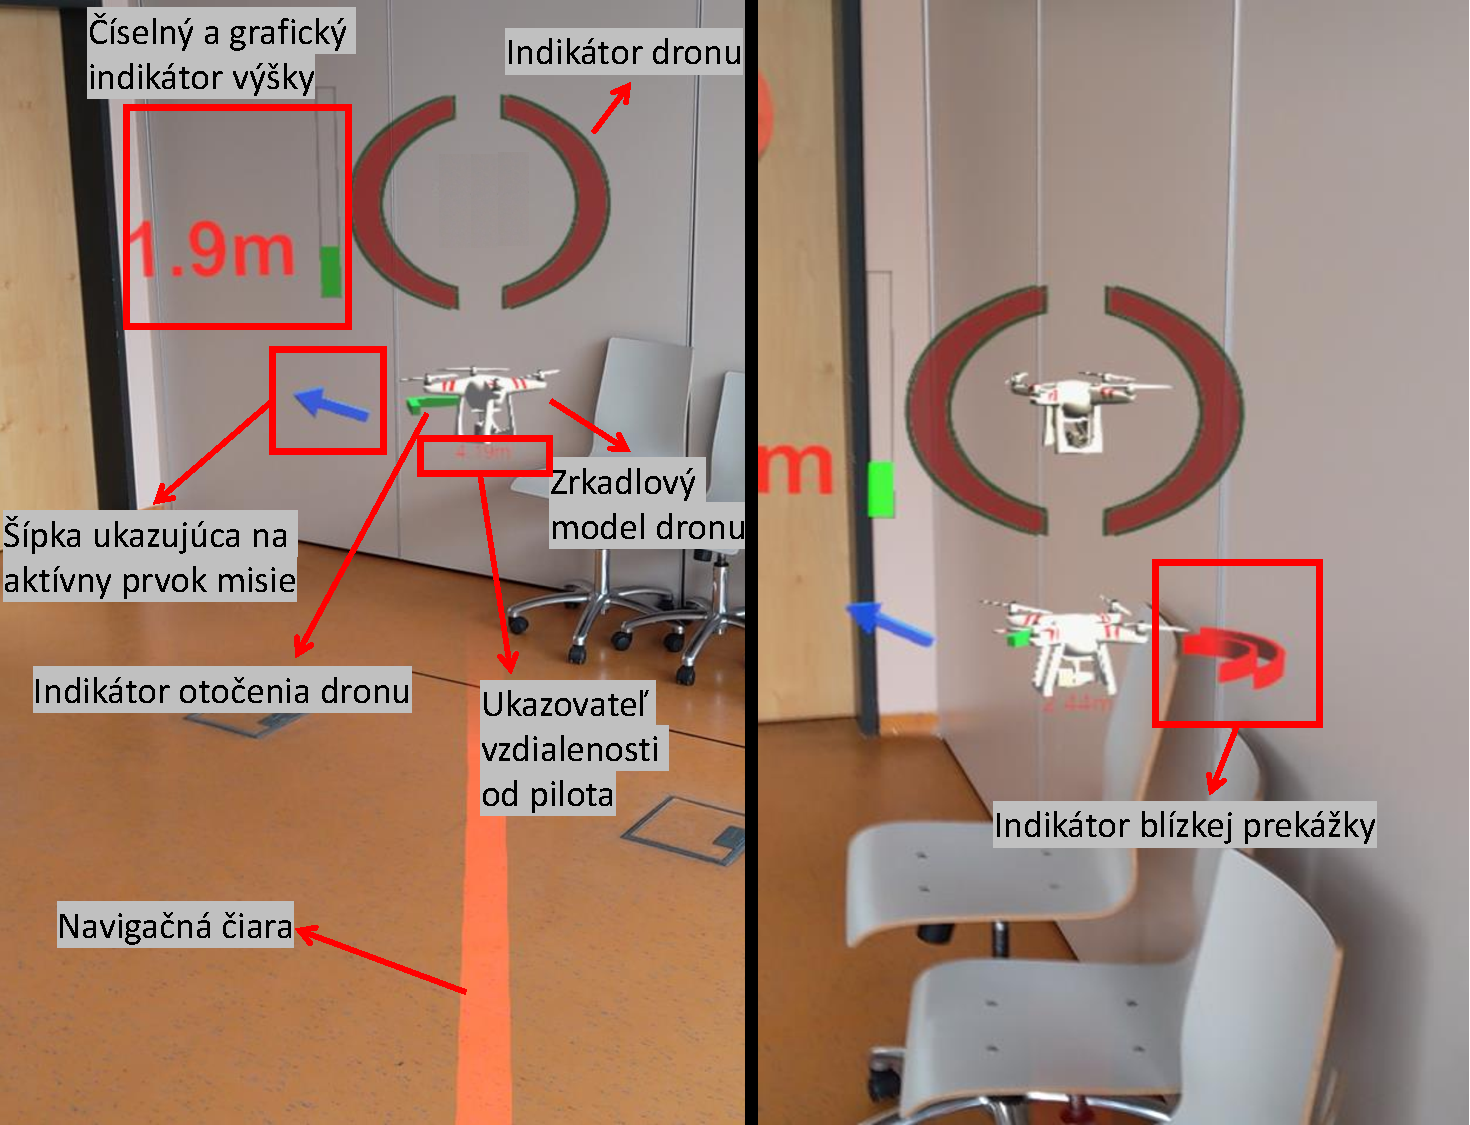
\includegraphics[width=0.77\textwidth]{obrazky-figures/navrh/prevUiDesign.pdf}
	\caption{Původní implementace vizualizace letových veličin. Převzato z práce \cite{KyjacMartin2022Vnpp}.}
	\label{pic:prevUiDesign}
\end{figure}


\begin{figure}[ht]
	\centering
	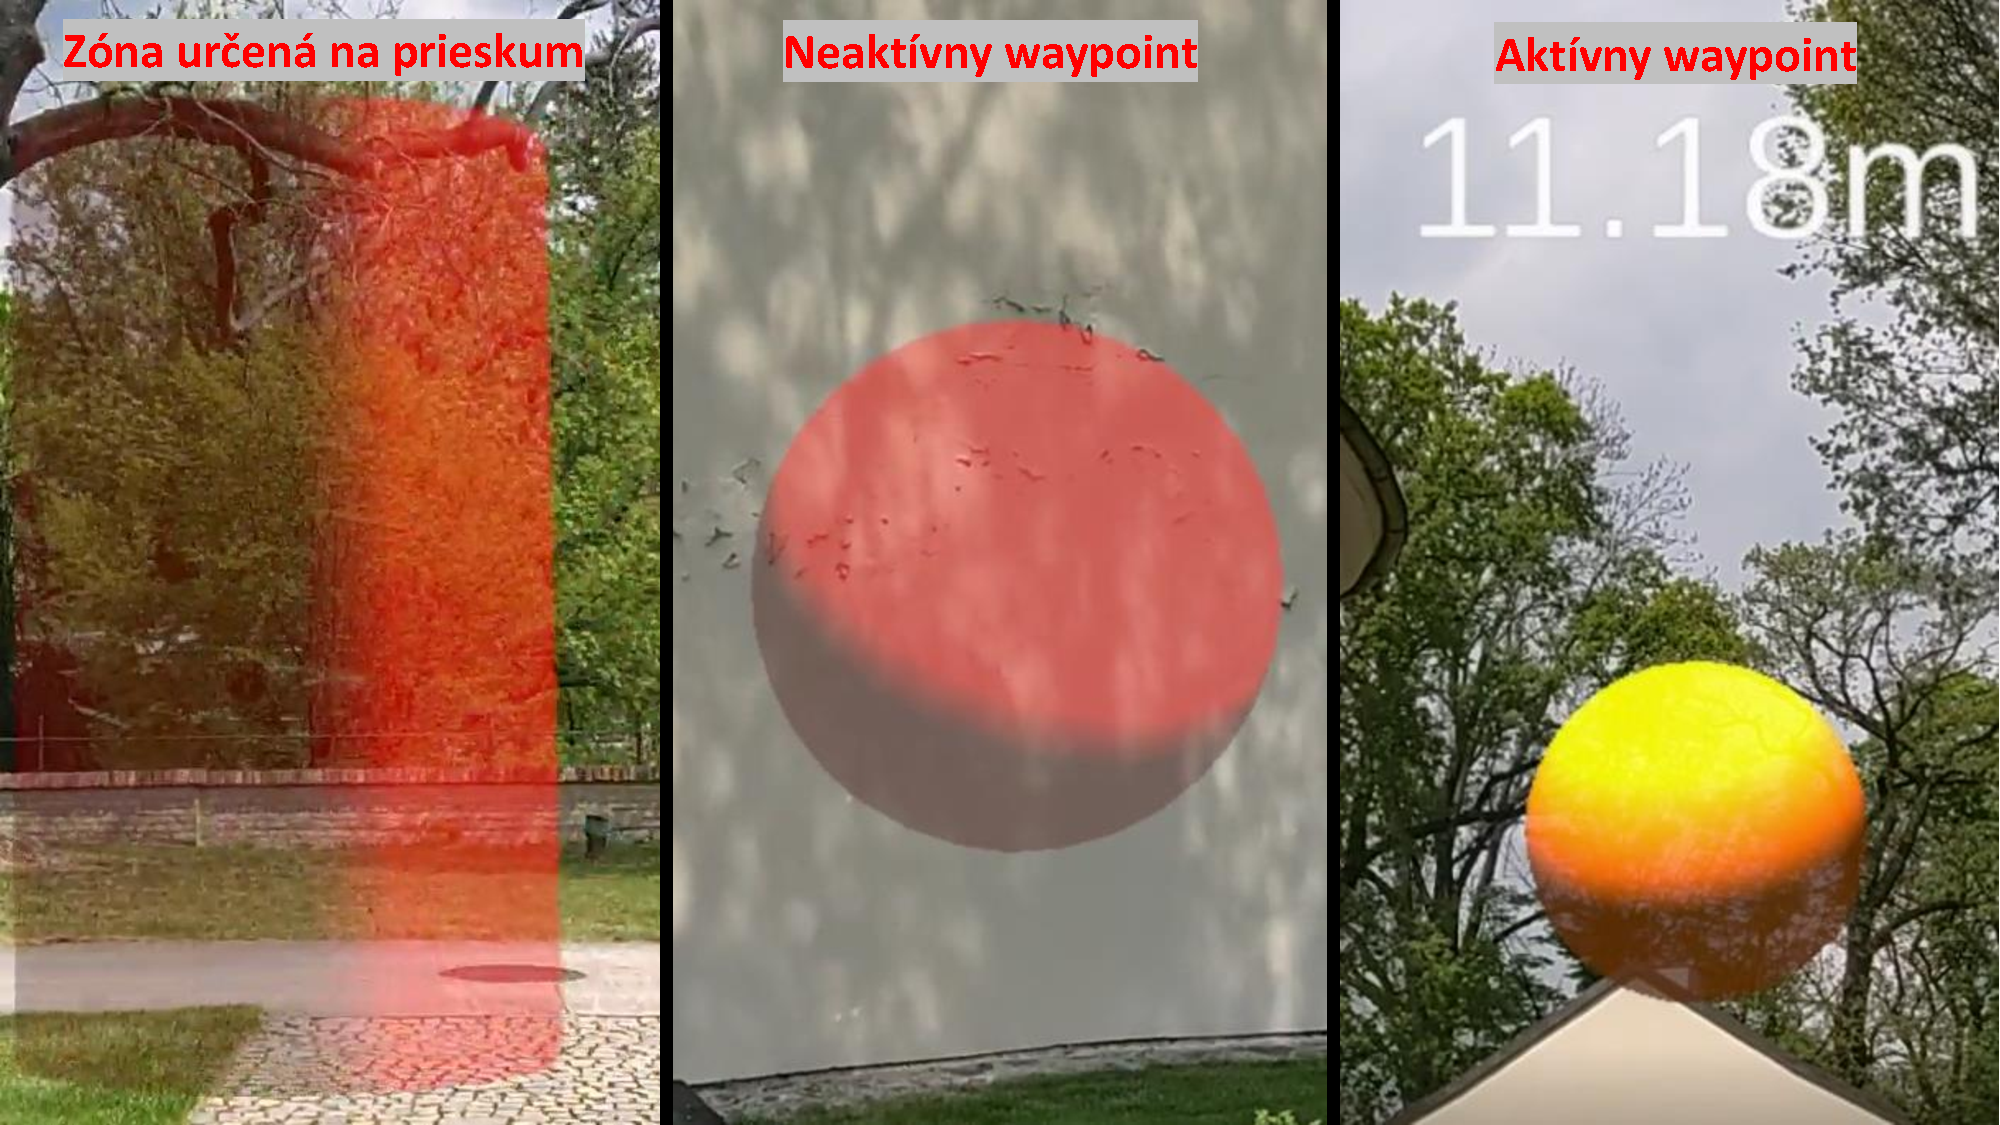
\includegraphics[width=0.76\textwidth]{obrazky-figures/navrh/prevMisionObject.pdf}
	\caption{Původní implementace objektů mise. Převzato z práce \cite{KyjacMartin2022Vnpp}.}
	\label{pic:prevMisionObject}
\end{figure}

\section{Požadavky nového řešení}
Sekce je zaměřena na shrnutí cílů a požadavků na novou implementaci rozhraní. Nejdříve budou shrnuty obecné požadavky a jak je plánované jejich docílení. 

\begin{itemize}
    \item Bezpečnost a soulad z legislativou - cílem nového řešení je usnadnit pilotovi pilotáž 
    
    \item Minimalizace přepínání kontextu - rozhraní by mělo nahradit telefon v ovladači, aby se nemusel často měnit pozornost pilota

    \item Větší imerze do letu
    
    \item Využití konceptů užitých v aktuálních leteckých přístrojích 
    
    \item Zvýšení povědomosti o okolí drona
    
    \item Implementace přenosu z kamery dronu.
    
    \item Předletová příprava a plánování mise 
    
    \item Intuitivnost rozhraní

    
    
    \item Využití 3D prostoru a lepší orientace v prostoru
    
\end{itemize}

\section{Drátové modely} % to do: přepsat kvůli autoplagiátorství
Drátové modely obvykle slouží pro vyjasnění polohy jednotlivých prvků rozhraní a~ne  pro vyobrazení grafické reprezentace, jak by mohlo na první pohled budit dojem. Drátové modely mají různé úrovně propracovanosti tak, aby mohly splnit účel, pro který jsou vytvořené.

Základní modely se obvykle skládají z~čar jedné barvy a~text má pouze umělecký charakter. Tyto modely jsou vhodné pro vyjasnění rozmístění jednotlivých prvků a sjednocení přístupů jednotlivých vývojářů. Vzhledem k~trivialitě těchto modelů se případné změny v~nich dají provést velmi snadno.

Propracovanější modely mohou mít stejný obsah, jako bude v~konečné reprezentaci rozhraní. Tento obsah může mít i~propracovanější rysy podobné jako u konečného produktu. Uvedené modely se často vytváří jako proklikávací (modely mají implementovanou základní funkčnost). Díky poslední zmíněné vlastnosti se s~uživateli dá provádět testování už v~návrhové části projektu a~získat tím cennou zpětnou vazbu ještě před dokončením skutečného prototypu~\cite{Wireframing,KomárekJakub2022Nzps}.

Vzhledem k~povaze projektu byl zvolen model odlehčenějšího charakteru. Autor vytvořil několik základních konceptů, které poté porovnal a~vybral nejlepší adepty pro další analýzu. Uvedené koncepty byly vytvořeny v~papírové podobě.


\todo{Jednotlivé wireframové návrhy}
\newpage
\section{Grafické modely}
Grafický návrh se naopak od drátového modelu soustředí na vizuální stránku rozhraní. V~této fázi návrhu je důležité vyjasnit fundamentální barevné kombinace a motivy v rozhraní \cite{KomárekJakub2022Nzps}. 

Pro tento účel byl použit nástroj Microsoft Paint 3D. Tento nástroj poskytuje jednoduché prostředí  pro tvorbu 3D objektů a jejich zasazení do scény. Zároveň ale podporuje jednoduché vkládání 2D objektů. Toho bylo využito při návrhu vizualizace letových veličin.
\todo{Jednotlivé grafické návrhy}

%\section{Zásady užité při návrhu}


\chapter{Implementace řešení}
Hlavní náplní kapitoly je realizace návrhu aplikace z předchozí kapitoly. Úvod kapitoly tvoří popis ekosystému v kterém má aplikace účinkovat. Součástí popisu je rozbor jednotlivých komponent, popis komunikace mezi nimi včetně popisu přenášených dat. Dále je navázáno představením technologií použitých při vývinu. Zbytek kapitoly je věnován detailnímu popisu implementačního procesu aplikace. Ten je rozdělen podle jednotlivých funkční modulů. Popis je doprovázen obrázkovou prezentací řešení.
\section{Architektura a komponenty systému } \label{sec:architektura}
Tato sekce se věnuje popisu celého ekosystému, který aplikace v brýlích potřebuje pro správné fungování. Systém bude nejdříve rozdělen a popsán podle jednotlivých komponentách. Na závěr bude nastíněna pravděpodobná hardwarová realizace v potencionální produkční verzi.

V systému účinkuje 7 komponent: Brýle, vysílač DJI\texttrademark, chytrý mobilní telefon, dron DJI\texttrademark, přístupový bod (dále již AP) a dvojice serverů (pro sběr a distribuci telemetrických dat a video streamů). Tyto komponenty jsou navzájem propojeny za pomocí různých přenosových technologií. Systém využívá serverového řešení z důvodu možnosti potencionálního budoucího rozšíření o integraci vizualizace více dronů či zapojení více operujících členů (například pozorovatelů).
Celý systém je vizualizován na obrázku \ref{pic:ekosystem}.
\paragraph{Popis jednotlivých komponent}
\begin{itemize}
    \item Brýle - Již představené brýle Hololens 2 pro rozšířenou realitu (viz. \ref{sec:Hololens}), které bude mít pilot po celou dobu pilotáže pilot nasazené. Brýle potřebují ke své funkci spojení s dvojicí serverů, od kterých jsou distribuovaná telemetrická data a video přenos. Přenos do brýlí probíhá za pomocí WI-FI přenosu z přístupového bodu. Právě zde bude nasazeno vyvíjené rozhraní. 
   
    \item Vysílač  DJI\texttrademark- Zajišťuje 3 hlavní funkce. První je bezdrátový přenos ovládacích instrukcí směrem k dronu a přenos telemetrických dat. K tomu využívá pásmo 2.4 GHz. Druhou funkcí je bezdrátový příjem video přenosu z kamery dronu. K tomu využívá pásmo 5 GHz. Oba zmíněné bezdrátové přenosy probíhají za pomocí proprietárních komunikačních technologií společnosti DJI\texttrademark. Třetí funkce ovladače je odesílání všech těchto dat do chytrého telefonu pomocí USB propoje. Více o vysílači viz. \ref{sec:ovladace}.
    
    \item Chytrý mobilní telefon - Jedná se o libovolný mobilní telefon se systémem android kompatibilní s vysílačem, ke kterému je připojen pomocí USB. V tomto telefonu musí být nainstalována  aplikace Drone DJI Streamer\footnote{Odkaz na aplikaci Drone DJI Streamer: \href{https://github.com/robofit/drone\_dji\_streamer}{github.com/robofit/drone\_dji\_streamer}}. 

    
    Jedná se o upravenou verze aplikace DJI Fly\footnote{Aplikace DJI Fly je oficiální aplikace pro pilotáž drona. Propojuje ovladač dronu s telefonem. Odkaz na aplikaci: \href{https://www.dji.com/cz/downloads/djiapp/dji-fly}{dji.com/cz/downloads/djiapp/dji-fly}  }, která je postavená na vydaném DJI SDK\footnote{SDK je soubor nástrojů, knihoven a dokumentace poskytovaných vývojářům pro snazší tvorbu aplikací. \\ Odkaz na DJI Android SDK: \href{https://developer.dji.com/mobile-sdk/downloads/}{developer.dji.com/mobile-sdk/downloads/}},  která zajistí distribuci telemetrických dat a video přenosu na patřičné servery. Uvažovaný způsob přenosu je pomocí technologie WI-FI přes přístupový bod. 
   
    \item Dron DJI\texttrademark \space - Obyčejný, softwarově neupravený dron od firmy DJI\texttrademark, který komunikuje s vysílačem. V práci byl použit dron DJI Mavic 2 mini.
   
    \item Přístupový bod - Zajišťuje propojení většiny koncových zařízení pomocí technologie WI-FI.
    
    \item Video server - Zajišťuje příjem a distribuci RTMP streamů, které jsou vysílány z z aplikace mobilního telefonu. V práci je využita serverová aplikace MonaServer\footnote{Odkaz na open-source implementaci serverové aplikace pro streamování RTMP přenosů videa: \\ \href{https://github.com/MonaSolutions/MonaServer}{github.com/MonaSolutions/MonaServer}}, která podporuje řadu streamovacích protokolů, mezi kterými je i požadovaný RTMP protokol.
   
    \item Telemetrický server - Zajišťuje příjem a distribuci telemetrických dat. V práci je využit již implementovaný DroCo server\footnote{Odkaz na DroCo server, který zajičtůje přenos telemetrických dat: \href{https://github.com/robofit/drone_server}{github.com/robofit/drone\_server}}. Tento server je určen na provoz v kontejnerovém prostředí Docker\footnote{Docker je open-source platforma pro balení a  spouštění aplikací v izolovaném prostředí pro zajištění konzistentní funkčnosti nehledě na konkrétní platformu systému.}.
\end{itemize}

\begin{figure*}[ht]
    \centering
    \includesvg[width=\linewidth]{obrazky-figures/architektura.svg}
    \caption{Obrázek ukazuje jednotlivé komponenty architektury systému  a  jejich vzájemné propojení. K dispozici je i legenda ukazující technologii  propoje. }
    \label{pic:ekosystem}
\end{figure*}

\subsection{Přenášená data}

\paragraph{Telemetrická data} - Přenášejí se mezi komponentami systému ve formátu JSON. Přenášejí se pouze nejnutnější data pro určení polohy, rychlosti pohybu a data pro režiji komunikace. Ukázka JSON dat viz. výpis \ref{drone-data-json}.
\paragraph{\textnormal{Popis jednotlivých údajů a veličin:}}
\begin{itemize}
    \item Client ID - Jedná se o jedinečný identifikátor v rámci jedné sítě. Jeden dron má právě přiřazen jeden tento identifikátor. Aplikace v telefonu si při registraci na server tento identifikátor vygeneruje. Jedná se o 8 znakový hexadecimální řetězec.
    \item  Altitude - Relativní výška dronu. Při startu dron předpokládá, že je ve výšce 0m. Potom pomocí akcelerometrů a optického senzoru odvozuje výšku, ve které se nachází. Znamená to, že pokud dron letí nad budovou, výška se nezmění.
    \item GPS souřadnice
    \begin{itemize}
        \item Latitude - Zeměpisná šířka ve stupních.
        \item Longitude - Zeměpisná délka ve stupních.
    \end{itemize}

    \item Údaje z gyroskopu - Jsou posílány dvakrát. Ve formě čistých dat z hlavního gyroskopu dronu a z gimbalu kamery. \todo{Doopravdy?}
    \begin{itemize}
        \item Pitch - Náklon kolem osy  ve stupních, která prochází zleva doprava středem dronu. Indikuje náklon dopředu/dozadu.
        \item Roll -  Náklon kolem osy  ve stupních, která prochází zezadu do předu středem dronu. Indikuje náklon doleva/doprava.
        \item Yew - Náklon kolem osy, která prochází z hora dolů  středem dronu. Indikuje otáčení dronu doleva/doprava.
    \end{itemize}
    \item Compass - Udává kurz dronu ve stupních. Měl by se shodovat s údajem Yew.
    \item Údaje z akcelerometů
    \begin{itemize}
        \item Velocity X - Dopředná rychlost v m/s
        \item Velocity Y - Horizontální rychlost (do leva/doprava) v m/s
        \item Velocity Z - Vertikální rychlost v m/s.
        %\item yaw_relative  - nevím co to je
     \end{itemize}
     \item Timestamp - Časová značka pořízení dat.
\end{itemize}

\begin{figure}[ht]
  \begin{minipage}{0.5\textwidth}
    \begin{lstlisting}[ caption={Ukázka telemetrických dat ve formátu JSON.}, label={drone-data-json}]
{
  "client_id": "15357fc2",
  "altitude": 221.5,
  "gps": {
    "latitude": 49.227189718704956,
    "longitude": 16.59724337395506
  },
  "aircraft_orientation": {
    "pitch": 2.7,
    "roll": 0.7,
    "yaw": -113.8,
    "compass": -113.80000305175781
  },
  "aircraft_velocity": {
    "velocity_x": 0,
    "velocity_y": 0,
    "velocity_z": 0
  },
  "gimbal_orientation": {
    "pitch": 0,
    "roll": 0,
    "yaw": -122.5999984741211,
    "yaw_relative": 0
  },
  "timestamp": "2023-09-06 15:58:58.999"
}
\end{lstlisting}
  \end{minipage}%
  \hfill
  \begin{minipage}{0.45\textwidth}
    \centering
    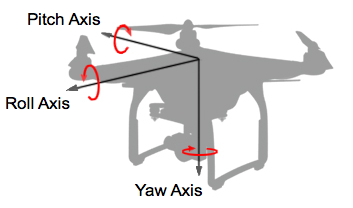
\includegraphics[width=\textwidth]{obrazky-figures/gymbal.png}
    \caption{Vizualizace náklonů, které lze vyčíst z gyroskopu. Převzato z \cite{Flight-Control-dji}. }
    \label{pic:gymbal}
    \vspace{20pt}
    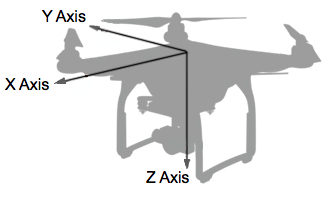
\includegraphics[width=\textwidth]{obrazky-figures/velocity.png}
    \caption{Vizualizace směrů rychlostí z akcelerometrů. Povšimněme si obrácené osy Z, která indikuje že rychlost při stoupání dronu je záporná. Převzato z \cite{Flight-Control-dji}.}
    \label{pic:velocity}
  \end{minipage}
\end{figure}
    
\paragraph{Video} - Video přenos z kamery dronu se přenáší za pomocí protokolu RTMP. Jedná se o protokol, který je používán pro přenos živého vysílání přes internet. Protokol rozděluje video stream do malých fragmentů, které následně posílá po síti. Protokol umí přenášet i audio stopu, pro tu však v práci není využití a proto je vypnuta. Tento protokol má přidělen TCP port 1935 a v čisté verzi není nijak zabezpečený\cite{RTMP}. 

Aplikace na telefonu dokáže zasílat živý přenos v HD rozlišení (1280x720 pixelů) při snímkovací frekvenci 30 snímků za sekundu. Užitý kodek je H264. Díky užití tohoto protokolu je zpoždění obrazu minimální.

\paragraph{Potencionální produkční implementace architektury}\mbox{} \\
Z předchozího popisu je patrné, že serverová část může být nasazena v internetu. Z praktického hlediska však tento přístup autor nedoporučuje kvůli velkým latencím při komunikaci a nepříliš velké variability v případě užití v terénu - řešení by bylo závislé na dosahu internetového spojení. 

Proto je uvažováno, že přístupový bod a obě serverové aplikace budou pravděpodobně integrovány v rámci jednoho systému a budou mít zajištěno externí napájení například z baterie. Celý tento systém by pak byl například umístěn do kufru pro přepravu drona. 

\paragraph{Vývojové prostředí architektury}\mbox{} \\
V rámci vývoje byl  systém integrován na vývojovém notebooku, který zastal funkci jak serveru, tak přístupového bodu. K vývoji značně dopomáhal vizualizační nástroj  DroCo\footnote{Odkaz na aplikaci DroCo: \href{https://github.com/robofit/drone\_vstool}{github.com/robofit/drone\_vstool}}, který vizualizoval data z obou serverů.

\section{Užité softwarové prostředky}
Tato práce navazuje na předchozí práci \cite{KyjacMartin2022Vnpp} a proto se autor rozhodl pokračovat na již zavedených softwarových prostředích. Hlavním stavebním kamenem je engine/framework Unity. V tomto enginu je celý program vytvářen. Dále autor využil několika doplňků/knihoven do tohoto enginu. Hlavní doplňky a knihovny budou popsány dále v této kapitole viz. \ref{}. 

Na tvorbu 3D objektů byl využit modelovací nástroj Blender. Ke tvorbě statické vektorové grafiky posloužil nástroj InkScape, který byl již popsán v návrhové části viz. \ref{}.  
\subsubsection{Unity}
Unity je multiplatformní herní Engine, který byl představen roku 2005. Tento engine byl primárně vytvořen pro tvorbu 2D a 3D her. Postupným vylepšováním a rozšířením se z něho stal univerzální nástroj pro tvorbu programů využívajících funkcionalit jádra tohoto enginu . Integraci enginu tak můžete nalézt například v automotive průmyslu, architektuře a stavebnictví.  

Jeho veliká výhoda spočívá ve snadné integraci aplikací na různé typy platforem. Standardně tak lze unity použít pro vývoj aplikací pro desktopy, mobilní telefony (Android + IOS), herní konzole, brýle pro VR/AR a nově i pro aplikace na Webu. Engine tak musí podporovat řadu architektur výpočetních systémů, což je v případě brýlý Hololens 2 potřeba (platforma ARM). 
\paragraph{C\#}
Tato platforma získala svou popularitu hlavně díky jednoduššímu a intuitivní stylu práce v tomto enginu. Jednoduché tvorbě dopomáhá jazyk C\#, který v enginu slouží pro psaní vnitřní logiky programu. Jedná se o vysokoúrovňový typovaný objektově orientovaný programovací jazyk. Tento jazyk lze mimo Unity nejčastěji nalézt v beckendové části Webových a formulářových aplikacích (.Net). 
\subsubsection{Blender}
Blender je opensource softwearový nástroj pro modelování 3D objektů, tvorbu animací a efektů. V kontextu práce je využívá pro editaci a tvorbu 3D objektů, které následně jsou zaneseny do 3D scény v Unity. 
\subsubsection{Git a Github}

\newpage
\section{Struktura programu}

\newpage
\section{Implementace jednotlivých části rozhraní}
\subsubsection{Statická část - vizualizace hlavních letových veličin}
\subsubsection{Dynamická část - sledování pozice dronu}
\subsubsection{Interaktivní mapa}


\chapter{Závěr semestrálního projektu}
Začátek práce je tvořen obeznámením s rozšířenou realitou. Dále jsou představeny brýle Hololens 2. Popsány jsou zejména modality vstupu brýlí a technické limitace brýlí. Téma další kapitoly byl drony a jejich bezpečný provoz dle legislativy. Navázalo se návrhem rozhraní v rámci kterého byla provedena analýza původního řešení. Poté následoval soupis požadavků nového rozhraní a stanovení cílů rozhraní. Dále bylo rozhraní navrhnuto pomocí drátových modelů a detaily doladěny v grafickém modelu. 

Závěr semestrálního projektu tvoří začátek implementační fáze projektu, kde byla prezentována architektura celého systému v rámci které byly popsány data, která se mezi jednotlivými systémy přenáší. V další sekci se již probíraly prostředky použité k vývoji. Poté byla od prezentována struktura programu, za kterou následoval popis implementace jednotlivých částí programu. 

V rámci pokračování práce chce autor dodělat všechny moduly popsané v návrhové části. Celý program chce autor uživatelsky otestovat, aby se ověřilo splnění cílů rozhraní udaných v návrhové části. Pro toto testování autor plánuje vytvořit testovací scénář v rámci kterého bude testovaný provádět řadu letových úkonů. Na konci testu bude testovaný vyplňovat řadu formulářů, mezi kterými bude NASA-TLX. Autor v rámci testování také chce měřit metriky jako je čas provádění úkonů a přesnost. Závěr diplomové práce má tvořit reprezentace výsledků testů a zodpovězení otázky, zadali technologie rozšířené reality má potenciál v tomto technologickém odvětví.

Pokud to časový rozpočet dovolí, autor by chtěl na závěr vložit rozpravu o možných budoucích směrech v této oblasti.

\begin{comment}
\chapter{Experimenty a uživatelské testování prototypu}
\section{Testovací scénář}
\section{Zhodnocení výsledků}
\subsection{NASA-TLX}
\subsection{Měřené veličiny}
\subsection{Testovací formulář}
\chapter{Možné budoucí směry a vývoj}
\section{Vývoj rozšířené reality}
- ukončení vývoje hololeans
- aplle? , ostatní hráči  na trhu....
\section{Vývoj vizualizace dronu}
\chapter{Závěr}

\end{comment}
